\chapter{Deep Learning Architectures}
\label{ch:models}

\section{Basic Concepts}
\label{sec:basic_concepts}
\emph{\ml} is a field of computer science that uses statistical techniques to allow computers to learn without being explicitly programmed.
\emph{\dl} is a subfield of \ml focusing on the use of neural networks~\footnote{In some papers, they emphasize the difference between neural networks and \emph{artificial neural networks} since we are not interested in studying \emph{human neural networks}, we will only be using the term neural networks.}.
The conceptual difference between \ml and \dl is:
\begin{center}
    \emph{\textbf{Machine Learning} is about learning general features. \\ \textbf{Deep Learning} is about learning abstract concepts.}
\end{center}

To emphasize the difference even more, consider \bdt (see for example \cite{bdt}), which is an old-fashioned \ml model, and \trans (see \cref{sec:transformer}), a modern \dl model. 
In the context of particle physics, \bdt is trained to provide learned cuts on the input data to separate the signal from the background.
On the other hand, \trans is learned to form an \emph{abstract representation} of the input data, from which one can extract information about the signal/background (this is even more apparent in \ParT and \depart, see \cref{sec:part,sec:depart}).
They can learn the differences between signal and background and \emph{general physical concepts} \cite{qcd_as_nlp}. 

\dl builds from the \mlp \cite{mlp}, a multi-layered neural network able to learn a \emph{any} non-linear function from input data.
In detail, we will discuss more enhanced \mlp in \cref{sec:fc}.

The general idea of \dl is to have some model, which is a set of parameters and functions, taking a set of inputs and producing a set of outputs.
The model is trained by adjusting the parameters to fit the desired outputs.
In this context, we are interested in the \emph{supervised} learning \cite{deeplearningbook}, where the desired outputs are known (\MC simulations, for example).
Some new use cases exist for \emph{self-supervised} learning \cite{masked_autoencoders}, where the desired outputs are unknown, but we will only briefly touch on them as a prospect.

\subsection{Forward and Backward Passes}
\label{sec:forward_backward}
Let $\pmb{x}$ be the input (generally a multi-dimensional tensor\footnote{This is NOT the same tensor as a physical tensor, which has a prescribed way of transforming, but rather a multi-dimensional array of numbers.}) of a model  $f(\bullet;\pmb{w})$ with trainable parameters $\pmb{w}$.
We will call the \emph{forward pass} of the model an application of the model on the input data $\pmb{o} = f(\pmb{x};\pmb{w})$, where $\pmb{o}$ is the output of the model (inference on input data $\pmb{x}$).
The \emph{backward pass} or \emph{backpropagation}\footnote{Term backpropagation comes from the application of the chain rule. Imagine the model as a composite of many functions, as the derivatives of the loss wrt. some parameters are computed, the chain rule is used to get \emph{back} to that parameter.} is the process of adjusting the parameters $\pmb{w}$ to fit the desired output $\pmb{y}$.
This is done by calculating the \emph{loss} $L(\pmb{o},\pmb{y})$ between the output $\pmb{o} = f(\pmb{x};\pmb{w})$ and the desired output $\pmb{y}$ (\emph{target}), and then adjusting the parameters $\pmb{w}$ to minimize the loss.
Loss is a measure of how far the model is from the target.

There are several ways of adjusting the parameters, but the widely used approaches are based on computing the gradient of the loss wrt. the parameters $\pmb{w}$ and then updating the parameters in the direction of the gradient \cite{deeplearningbook}. 
This can be sketched as follows
\begin{equation}
    \pmb{w} \leftarrow \pmb{w} - \alpha \cdot \mathcal{O}\left[\nabla_{\pmb{w}} L(f(\pmb{x};\pmb{w}),\pmb{y})\right],
\end{equation}
where $\alpha$ is the \emph{learning rate} and $\mathcal{O}$ is the optimization algorithm (function), shortly \emph{optimizer}.
 The loss is usually calculated on a \emph{batch} of data, making the process more efficient and parallelizable,  which is then averaged to get the final loss
\begin{equation}
    \pmb{w} \leftarrow \pmb{w} - \alpha \cdot \mathcal{O}\left[ \nabla_{\pmb{w}} \frac1B \sum_{i=1}^B L(f(\pmb{x}^{(i)};\pmb{w}),\pmb{y}^{(i)})\right],
\end{equation}
where $B$ is the batch size and $\pmb{x}^{(i)}$ and $\pmb{y}^{(i)}$ are the $i$-th elements of the batch.

\subsection{Traning process}
\label{sec:training_process}
Before discussing the individual models, we will briefly touch on the training process as a whole.

The dataset is split into a \emph{training set}, a \emph{validation set}, and in our case, also a \emph{test set}.
The training set is used to train the model, the validation set is used to monitor the training process, and the test set is used to evaluate the model's performance.
The training process is split into several \emph{epochs}, each consisting of several \emph{iterations}.
An epoch is a complete pass through the training data, while an iteration is a single batch of data.
The total number of \emph{steps} is the product of the number of epochs and iterations. 

After each epoch, we evaluate the model on the training set and the validation set.
Validation is done to have a statistically independent measure of the model's performance during the training process.


\subsection{Output layer}
\label{sec:output_layer}
Based on the type of the target output, we can distinguish between \emph{regression} and \emph{classification} problems.

\textbf{classification} is the task of predicting a discrete variable.
The model's output is a vector of numbers $\pmb{v}$, where the length of the vector is the number of classes.
It is a \emph{one-hot} encoded vector, meaning that the index of the non-zero element is the desired class.
To perform a classification task, we must convert the vector $\pmb{v}$ into a probability distribution over the classes.
This is done by applying the \emph{softmax} function to the vector $\pmb{v}$, which is defined as
\begin{equation}
    \pmb{p} = \mathrm{softmax}(\pmb{v}) = \frac{\exp(\pmb{v})}{\sum_{i=1}^N \exp(v_i)},
\end{equation}
where $N$ is the number of classes.
In a case of binary classification (only two classes), the vector is a single number $v$, and the softmax function reduces to a \emph{sigmoid} function
\begin{equation}
    p = \sigma(v) = \frac{1}{1 + \exp(-v)}.
\end{equation}
Ideally, we would like the vector $\pmb{v}$ to have a single non-zero element corresponding to the correct class. 
In the case of binary classification, we would like the number $v$ to be either zero or one.

\textbf{regression} is the task of predicting a continuous variable.
The model's output is a vector of numbers $\pmb{v}$, where the length of the vector is the number of variables to be predicted.
There is no output layer function for regression.


\subsection{Loss Functions}
\label{sec:loss_functions}
The loss function measures how far the model is from the target.
In the old days of \ml, the most common loss function was the \MSE, defined as 
\begin{equation}
    \label{eq:MSE}
    L(\pmb{o},\pmb{y}) = \frac{1}{N} \sum_{i=1}^N (o_i - y_i)^2,
\end{equation}
where $N$ is the number of variables to be predicted (number of classes, in case of classification task).

In modern \dl frameworks, the \emph{cross-entropy} loss is the most common loss function, rooting from the \emph{information theory}.
To briefly introduce cross-entropy loss, we will introduce some basic concepts from information theory \cite{shannon}.
We will denote the probability of a random variable $x \in X$ by $p(x)$, where $X$ is the set of all possible values of the random variable.
\begin{description}
    \item [Self-information] of a random variable $x$ is defined as
    \begin{equation}
        I_p(x) = \log \frac{1}{p(x)} =- \log p(x).
    \end{equation}
    The self-information measures the \emph{surprise} of obtaining random variable $x$ when sampled from $p$.
    \item[Entropy] of distribution $p$ is defined as a mean self-information of the distribution
    \begin{equation}
        H(p) = \left< I_p(x)\right>_p = - \sum_{x \in X} p(x) \log p(x).
    \end{equation}
    The entropy measures the \emph{average surprise} of obtaining a random variable from the distribution $p$.
    The entropy is zero if the random variables are deterministic and maximal if the random variables are uniformly distributed.
    \item[Cross-entropy] is defined as a mean value of the self-information of the distribution $q$ when sampled from the distribution $p$
    \begin{equation}
        H(p,q) = \left< I_q(x)\right>_p = - \sum_{x \in X} p(x) \log q(x).
    \end{equation}
    The cross-entropy measures the \emph{average surprise of distribution $q$} when the actual distribution is $p$.
    Because of the \emph{Gibbs inequality} $H(p,q) \geq H(p)$, \cite{information_theory}, the cross-entropy is minimal if the distribution $q$ is equal to the distribution $p$.
    \item[Kullback-Leibler (KL) divergence] is a difference between the cross-entropy of the distribution $p$ and $q$ and the entropy of the distribution $p$.
    \begin{equation}
        D_{\text{KL}}(p|q) =  H(p,q) - H(p) = - \sum_{x \in X} p(x) \log \frac{p(x)}{q(x)}.
    \end{equation}
    The KL divergence measures the \emph{excess of the average surprise of distribution $p$} when the actual distribution is $p$.
\end{description} 

We can now define the \emph{cross-entropy loss} function
\begin{equation}
    \label{eq:cross_entropy}
    L(\pmb{o},\pmb{y}) = - \sum_{i=1}^N y_i \log o_i.
\end{equation}
It is important to note that cross-entropy is defined for probability distributions so that the cross-entropy loss can be used only for classification tasks.

This is an excellent place to discuss the similarities to physical entropy.
In modern statistical physics, the definition of classical entropy roots exactly from Shannon \cite{shannon} as in the information theory.
It is the \emph{measure of ignorance}, in the sense of missing information.
In this context, we can say that the cross-entropy is the \emph{measure of ignorance} of the model.
In quantum mechanics, entropy was developed by John von Neumann \cite{VonNeumann}, where the definition is slightly different, but it is the same regarding probability distributions.
The KL divergence is precisely the \emph{measure of the distinguishability of two quantum states}.


\subsection{Optimizers}
\label{sec:optimizers}
\emph{Optimizers} are algorithms that adjust the model weights to minimize the loss function.
The most common optimizers are based \emph{gradient descent} and its variants \cite{optimization}.
All of them have a common hyperparameter, the \emph{learning rate} $\alpha$, which controls the size of the steps taken by the optimizer.
We introduce three common optimizers: 
\begin{description}
    \item[SGD] (\emph{Stochastic Gradient Descent}) \cite{deeplearningbook} is an old-school \ml algorithm.
    \begin{algorithm}
        \begin{algorithmic}
        \Require model with weights $f(\bullet;\pmb{w})$, outputs of a model $f(\pmb{x}^{(i)};\pmb{w})$ in batches, target values $\pmb{y}^{(i)}$ in batches
        \Require learning rate $\alpha$
        \For{n = 1 \textbf{to} \texttt{number of iterations}}
            \State $\pmb{g} \gets \nabla_{\pmb{w}} \frac1B \sum_{i=1}^B L(f(\pmb{x}^{(i)};\pmb{w}),\pmb{y}^{(i)})$
            \State $\pmb{w} \gets \pmb{w} - \alpha \pmb{g}$
        \EndFor
        \Ensure model $f(\bullet;\pmb{w})$ with optimized weights $\pmb{w}$
        \end{algorithmic}
        \caption{SGD}
        \label{alg:sgd}
    \end{algorithm}
    \item[Adam] (\emph{Adaptive Moment Estimation}) \cite{adam} is a popular \dl algorithm used in almost every \dl framework.
    As hyperparameters, apart from the learning rate $\alpha$, it has the decay rate of the first moment $\beta_1$, the decay rate of the second moment $\beta_2$, a small constant $\epsilon$ to avoid division by zero, and weight decay $\lambda$ (which we will explain in \cref{sec:regularization}).
    \begin{algorithm}
        \begin{algorithmic}[1]
        \Require model with weights $f(\bullet;\pmb{w})$, outputs of a model $f(\pmb{x}^{(i)};\pmb{w})$ in batches, target values $\pmb{y}^{(i)}$ in batches
        \Require learning rate $\alpha$, decay rate of the first moment $\beta_1$, decay rate of the second moment $\beta_2$, small constant $\epsilon$, weight decay $\lambda$
        \For{n = 1 \textbf{to} \texttt{number of iterations}}
            \State $\pmb{g} \gets \nabla_{\pmb{w}} \frac1B \sum_{i=1}^B L(f(\pmb{x}^{(i)};\pmb{w}),\pmb{y}^{(i)})$
            \State $\pmb{s} \gets \beta_1 \pmb{s} + (1 - \beta_1) \pmb{g}$
            \State $\pmb{r} \gets \beta_2 \pmb{r} + (1 - \beta_2) \pmb{g}^2$
            \State $\pmb{s} \gets \frac{\pmb{s}}{1 - \beta_1^n}$
            \State $\pmb{r} \gets \frac{\pmb{r}}{1 - \beta_2^n}$
            \State $\pmb{m} \gets \frac{\pmb{s}}{\sqrt{\pmb{r}} + \epsilon} + \lambda \pmb{w}$
            \State $\pmb{w} \gets \pmb{w} - \alpha \pmb{m}$
        \EndFor
        \Ensure model $f(\bullet;\pmb{w})$ with optimized weights $\pmb{w}$
        \end{algorithmic}
        \caption{Adam}
        \label{alg:adam}
    \end{algorithm}
    There are several notable differences between Adam and SGD.
    First, Adam uses the \emph{momentum} (remembering the size of the previous step) to accelerate the convergence, which is represented by the addition of $\beta_1\pmb{s}$ in line 3 of \cref{alg:adam}.
    Second, Adam uses the \emph{adaptive learning rate} to avoid the problem of the learning rate being too low or too large, which is represented by the division of $\sqrt{\pmb{r}}$ in line 7 of \cref{alg:adam}.
    Adam uses the second moment $\pmb{g}^2$, line 4 of \cref{alg:adam} to calculate the adaptive learning rate.
    The operations in lines 5 and 6 of \cref{alg:adam} are called \emph{bias correction}.
    \item[LAMB] (\emph{Layer-wise Adaptive Moments optimizer for Batch training}) \cite{lamb} is a state-of-the-art \dl algorithm built upon Adam, which helps train large models.
    It has the same hyperparameters as Adam.
    \begin{algorithm}
        \begin{algorithmic}[1]
        \Require model with weights $f(\bullet;\pmb{w})$, outputs of a model $f(\pmb{x}^{(i)};\pmb{w})$ in batches, target values $\pmb{y}^{(i)}$ in batches
        \Require learning rate $\alpha$, decay rate of the first moment $\beta_1$, decay rate of the second moment $\beta_2$, small constant $\epsilon$, weight decay $\lambda$
        \For{n = 1 \textbf{to} \texttt{number of iterations}}
            \State $\pmb{g} \gets \nabla_{\pmb{w}} \frac1B \sum_{i=1}^B L(f(\pmb{x}^{(i)};\pmb{w}),\pmb{y}^{(i)})$
            \State $\pmb{s} \gets \beta_1 \pmb{s} + (1 - \beta_1) \pmb{g}$
            \State $\pmb{r} \gets \beta_2 \pmb{r} + (1 - \beta_2) \pmb{g}^2$
            \State $\pmb{s} \gets \frac{\pmb{s}}{1 - \beta_1^n}$
            \State $\pmb{r} \gets \frac{\pmb{r}}{1 - \beta_2^n}$
            \State $\pmb{m} \gets \frac{\pmb{s}}{\sqrt{\pmb{r}} + \epsilon} + \lambda \pmb{w}$
            \State $\pmb{w} \gets \pmb{w} - \alpha  \left\lVert \pmb{w} \right\rVert  \frac{m}{\left\lVert m \right\rVert}$
        \EndFor
        \Ensure model $f(\bullet;\pmb{w})$ with optimized weights $\pmb{w}$
        \end{algorithmic}
        \caption{LAMB}
        \label{alg:lamb}
    \end{algorithm}
    LAMB introduces the normalization of the step, which can be seen in line 8 of \cref{alg:lamb}.
    This normalization is done layer-wise to ensure that the weights will not diverge.
    The second improvement is the scaling based on the size of the weights, which can be seen in line 8 of \cref{alg:lamb} as $\left\lVert \pmb{w} \right\rVert$.
    Both normalizations are $l_2$-norms \cite{lamb}.
\end{description}

\subsubsection*{Learning Rate Scheduling}
\emph{Learning Rate Scheduling} is a process of changing the learning rate during the training process.
Usually, it is done as a decay of the learning rate to allow the model to converge into the absolute minimum of the loss function.
Let us denote the learning rate at the $n$-th iteration as $\alpha_n$ and $N$ as the total number of steps.
There are three common methods of learning rate decay: 
\begin{itemize}
    \item \textbf{Linear} $\alpha_n = \alpha_0\left(1-\frac{n}{N}\right)$,
    \item \textbf{Exponential} $\alpha_n = \alpha_0\cdot d^n$, where $d \in (0,1)$ is a number,
    \item \textbf{Cosine} $\alpha_n = \alpha_0\cdot\frac12\left(1+\cos\left(\frac{\pi n}{N}\right)\right)$.
\end{itemize}
\subsubsection*{Exploding Gradient}
Huge models tend to diverge, called \emph{exploding gradient}.
There are two common methods to prevent this \cite{deeplearningbook}:
\begin{itemize}
    \item \textbf{Gradient Clipping} allows a maximum value $c$ of the norm of the gradient $\left\lVert \pmb{g} \right\rVert$, if it is larger than $c$, it is scaled down to $c \frac{\pmb{g}}{\left\lVert \pmb{g} \right\rVert}$.
    \item \textbf{Warmup} is a method that increases the learning rate from zero to the desired value (usually linear) at the beginning of the training in some number of \emph{warmup steps}.
\end{itemize}

\subsection{Activation Functions}
\label{sec:activations}
\dl neural networks are composed of two types of operations: \emph{linear} and \emph{non-linear}.
Linear (more precisely, affine) operations are basic matrix multiplications.
Non-linear operations are the \emph{activation functions}, which are applied element-wise to the output of the linear operations.
Alternating between linear and non-linear operations is the key to the power of \dl neural networks, which can approximate \emph{any} function with enough layers and learned parameters.
A \emph{Universal Approximation Theorem} \cite{universal_app_thm} states that a simple \fc (see \cref{sec:fc}) with one hidden layer containing a finite number of neurons can approximate any continuous function on a compact subset of $\mathbb{R}^n$ to any desired accuracy.

In this section, we will briefly discuss the most common activation functions:
\begin{itemize}
    \item \textbf{tanh} - old-fashioned \ml activation \footnote{However it is still being used in \dl, for example in the RNN\cite{rnn}.} 
    \begin{equation}
        \tanh(x) = \frac{e^x - e^{-x}}{e^x + e^{-x}}
    \end{equation}
    \item \textbf{ReLU} (Rectified Linear Unit) - most common, 'goto' \dl activation 
    \begin{equation}
        \text{ReLU}(x) = \max(0,x),
    \end{equation}
    \item \textbf{GELU} (Gaussian Error Linear Unit) \cite{gelu} - smooth version of ReLU,  
    \begin{equation}
        \text{GELU}(x) = x\Phi(x) = x\frac{1}{2}\left(1 + \text{erf}\left(\frac{x}{\sqrt{2}}\right)\right),
    \end{equation}
    where $\Phi(x)$ is the cumulative distribution function of the standard normal distribution and $\text{erf}(x)$ is the error function,
    \item \textbf{Swish or SiLU} (Sigmoid Linear Unit) \cite{swish} - smooth version of ReLU, 
    \begin{equation}
        \text{Swish}(x) = x\sigma(x) = \frac{x}{1 + e^{-x}},
    \end{equation}
    \item \textbf{sigmoid} - after the last layer to convert a number to the probability 
    \begin{equation}
        \sigma(x) = \frac{1}{1 + e^{-x}},
    \end{equation}
    \item \textbf{Softmax} - after the last layer to convert a vector to a probability distribution 
    \begin{equation}
        \text{softmax}(\pmb{x}) = \frac{e^{\pmb{x}}}{\sum_{j=1}^n e^{x_j}}.
    \end{equation}
\end{itemize}
Sigmoid and Softmax were discussed in \cref{sec:output_layer}.
Graph with the activation functions can be seen in \cref{fig:activations} (softmax is excluded since in one dimension it reduces to sigmoid),
\begin{figure}[htb]
    \centering
    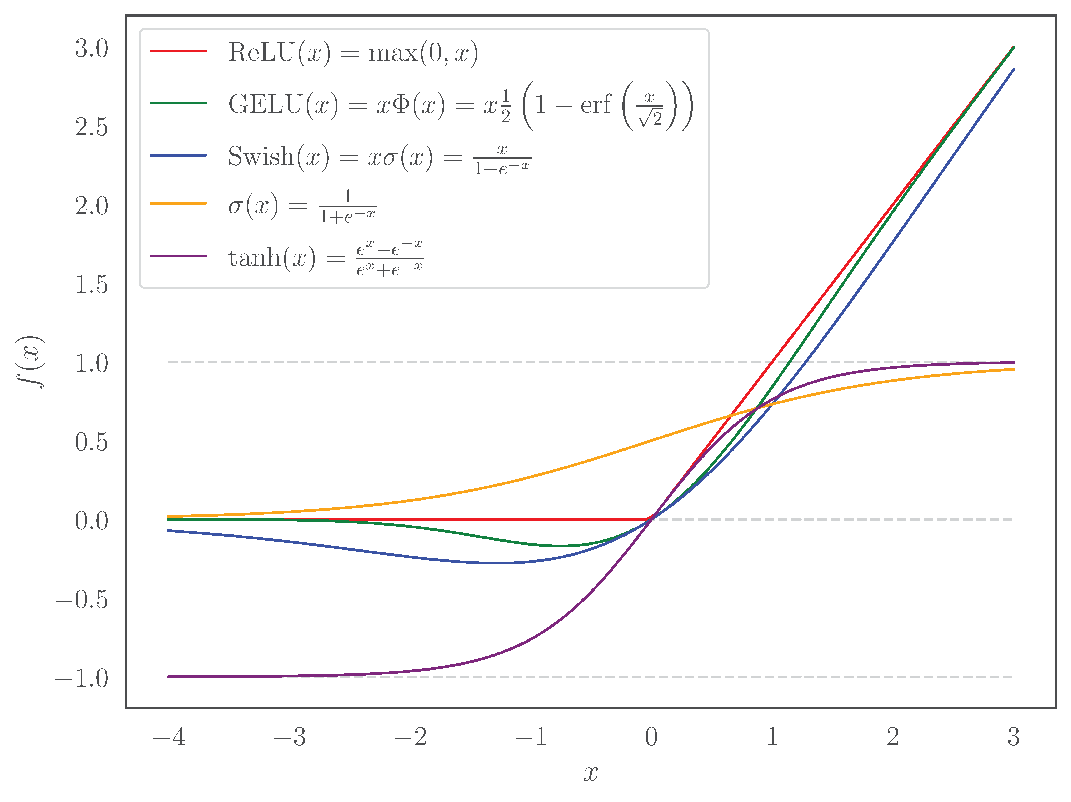
\includegraphics[width=1\linewidth]{src/img/activation_functions_a.pdf}
    \caption{Activation functions}
    \label{fig:activations}
\end{figure}

\subsection{Regularization}
\label{sec:regularization}
\textbf{Overfitting} happens when the model memorizes the training data instead of learning the underlying pattern, which is why we need the validation dataset to estimate the \emph{generalization error}.
\textbf{Underfitting} is the opposite when the model is not trained enough to capture the underlying pattern.
These terms are generally used across all \ml algorithms. 
Still, they are essential in \dl, where the number of parameters is much larger than the number of training examples (for example \cite{deit3,gpt3}).

Remarkably, deep networks performance \emph{increases} with the number of parameters.
There is a study \cite{double_descent} showing that if you pass the classical regime of 'Bias-Variance Tradeoff' (a more complex model with a lower bias but higher variance) with the number of parameters, the modern regime of 'Larger Model is Better' goes forever.
This is another proof of the statements in \cref{sec:basic_concepts} saying that \dl models can learn abstract concepts. 

However, to be able not to overfit the model, we need to use \textbf{regularization}. 
Regularization is a technique that prevents the model from overfitting by obstructing or penalizing the learning process.
We will list the most common regularization techniques:
\begin{description}
    \item[Weight decay] or \textbf{L2 regularization} is a penalty added to the loss function $l_2$-norm of the weights.
    \begin{equation}
        \label{eq:weight_decay}
        L \gets L + \lambda \left\lVert \pmb{w} \right\rVert^2,
    \end{equation}
    where $\lambda$ is the regularization strength.
    This regularization is usually implemented into the optimizer because the gradient can be explicitly calculated. 
    See \cref{sec:optimizers}. 
    \item[Dropout] is a technique that randomly sets some of the weights to zero \emph{during training}.  
    The probability of a weight being set to zero is the only hyperparameter.
    Dropout forces the network to learn different data representations and not rely on individual neurons.
    \item[Label smoothing] is a technique that replaces the one-hot encoded labels with a distribution of probabilities.
    For example, if the target is $\pmb{y} = (0., 1., 0.)$ (second class), and we set the hyperparameter of label smoothing to 0.1, the new label is $\tilde{\pmb{y}} = (0.1, 0.8, 0.1)$.
    \item[Augmentation] is a technique that applies random transformations to the input data.
    For example, if we have an image as an input, we can randomly rotate, crop, and change the brightness,
    \item[Ensambling] is a technique that combines multiple models into one by averaging their predictions.
\end{description}


\subsection{Metrics}
\label{sec:metrics}
A \emph{metric} measures how well the model performs. 
It \emph{evaluates} the model.
We will only discuss the metrics for binary classification since we will use that.
The output of a binary classification model is a single number between zero and one $o \in [0,1]$, where zero corresponds to the first class, and one corresponds to the second class.
We make a \emph{threshold} $T \in (0,1)$, where we assign the output to the first class if $o < T$ and to the second class if $o \geq T$. 
Usually, the threshold is set to 0.5, but it can be adjusted to optimize the desired output of the model.
Going further, we will assume that the threshold is set to 0.5 unless stated otherwise.

Let us denote the number of inputs that are correctly classified as the first class $T_0$, the number of events that are correctly classified as the second class $T_1$, the number of events that are incorrectly classified as the first class $F_0$, the number of events that are incorrectly classified as the second class $F_1$.
Usually, these quantities are denoted as \emph{true positives} (TP), \emph{true negatives} (TN), \emph{false positives} (FP), and \emph{false negatives} (FN), respectively.
However, they are confusing and refer to one class as positive and the other as negative, which is not the case in our binary classification, where both classes are equally important.
We try to simplify the notation by using the terms \emph{true} $T$ and \emph{false} $F$ to denote the correct and incorrect classification, respectively, and the numbers $0$ and $1$ to indicate the output class.
A diagram of these quantities is shown in \cref{fig:metrics}.
\begin{figure}[htb]
    \centering
    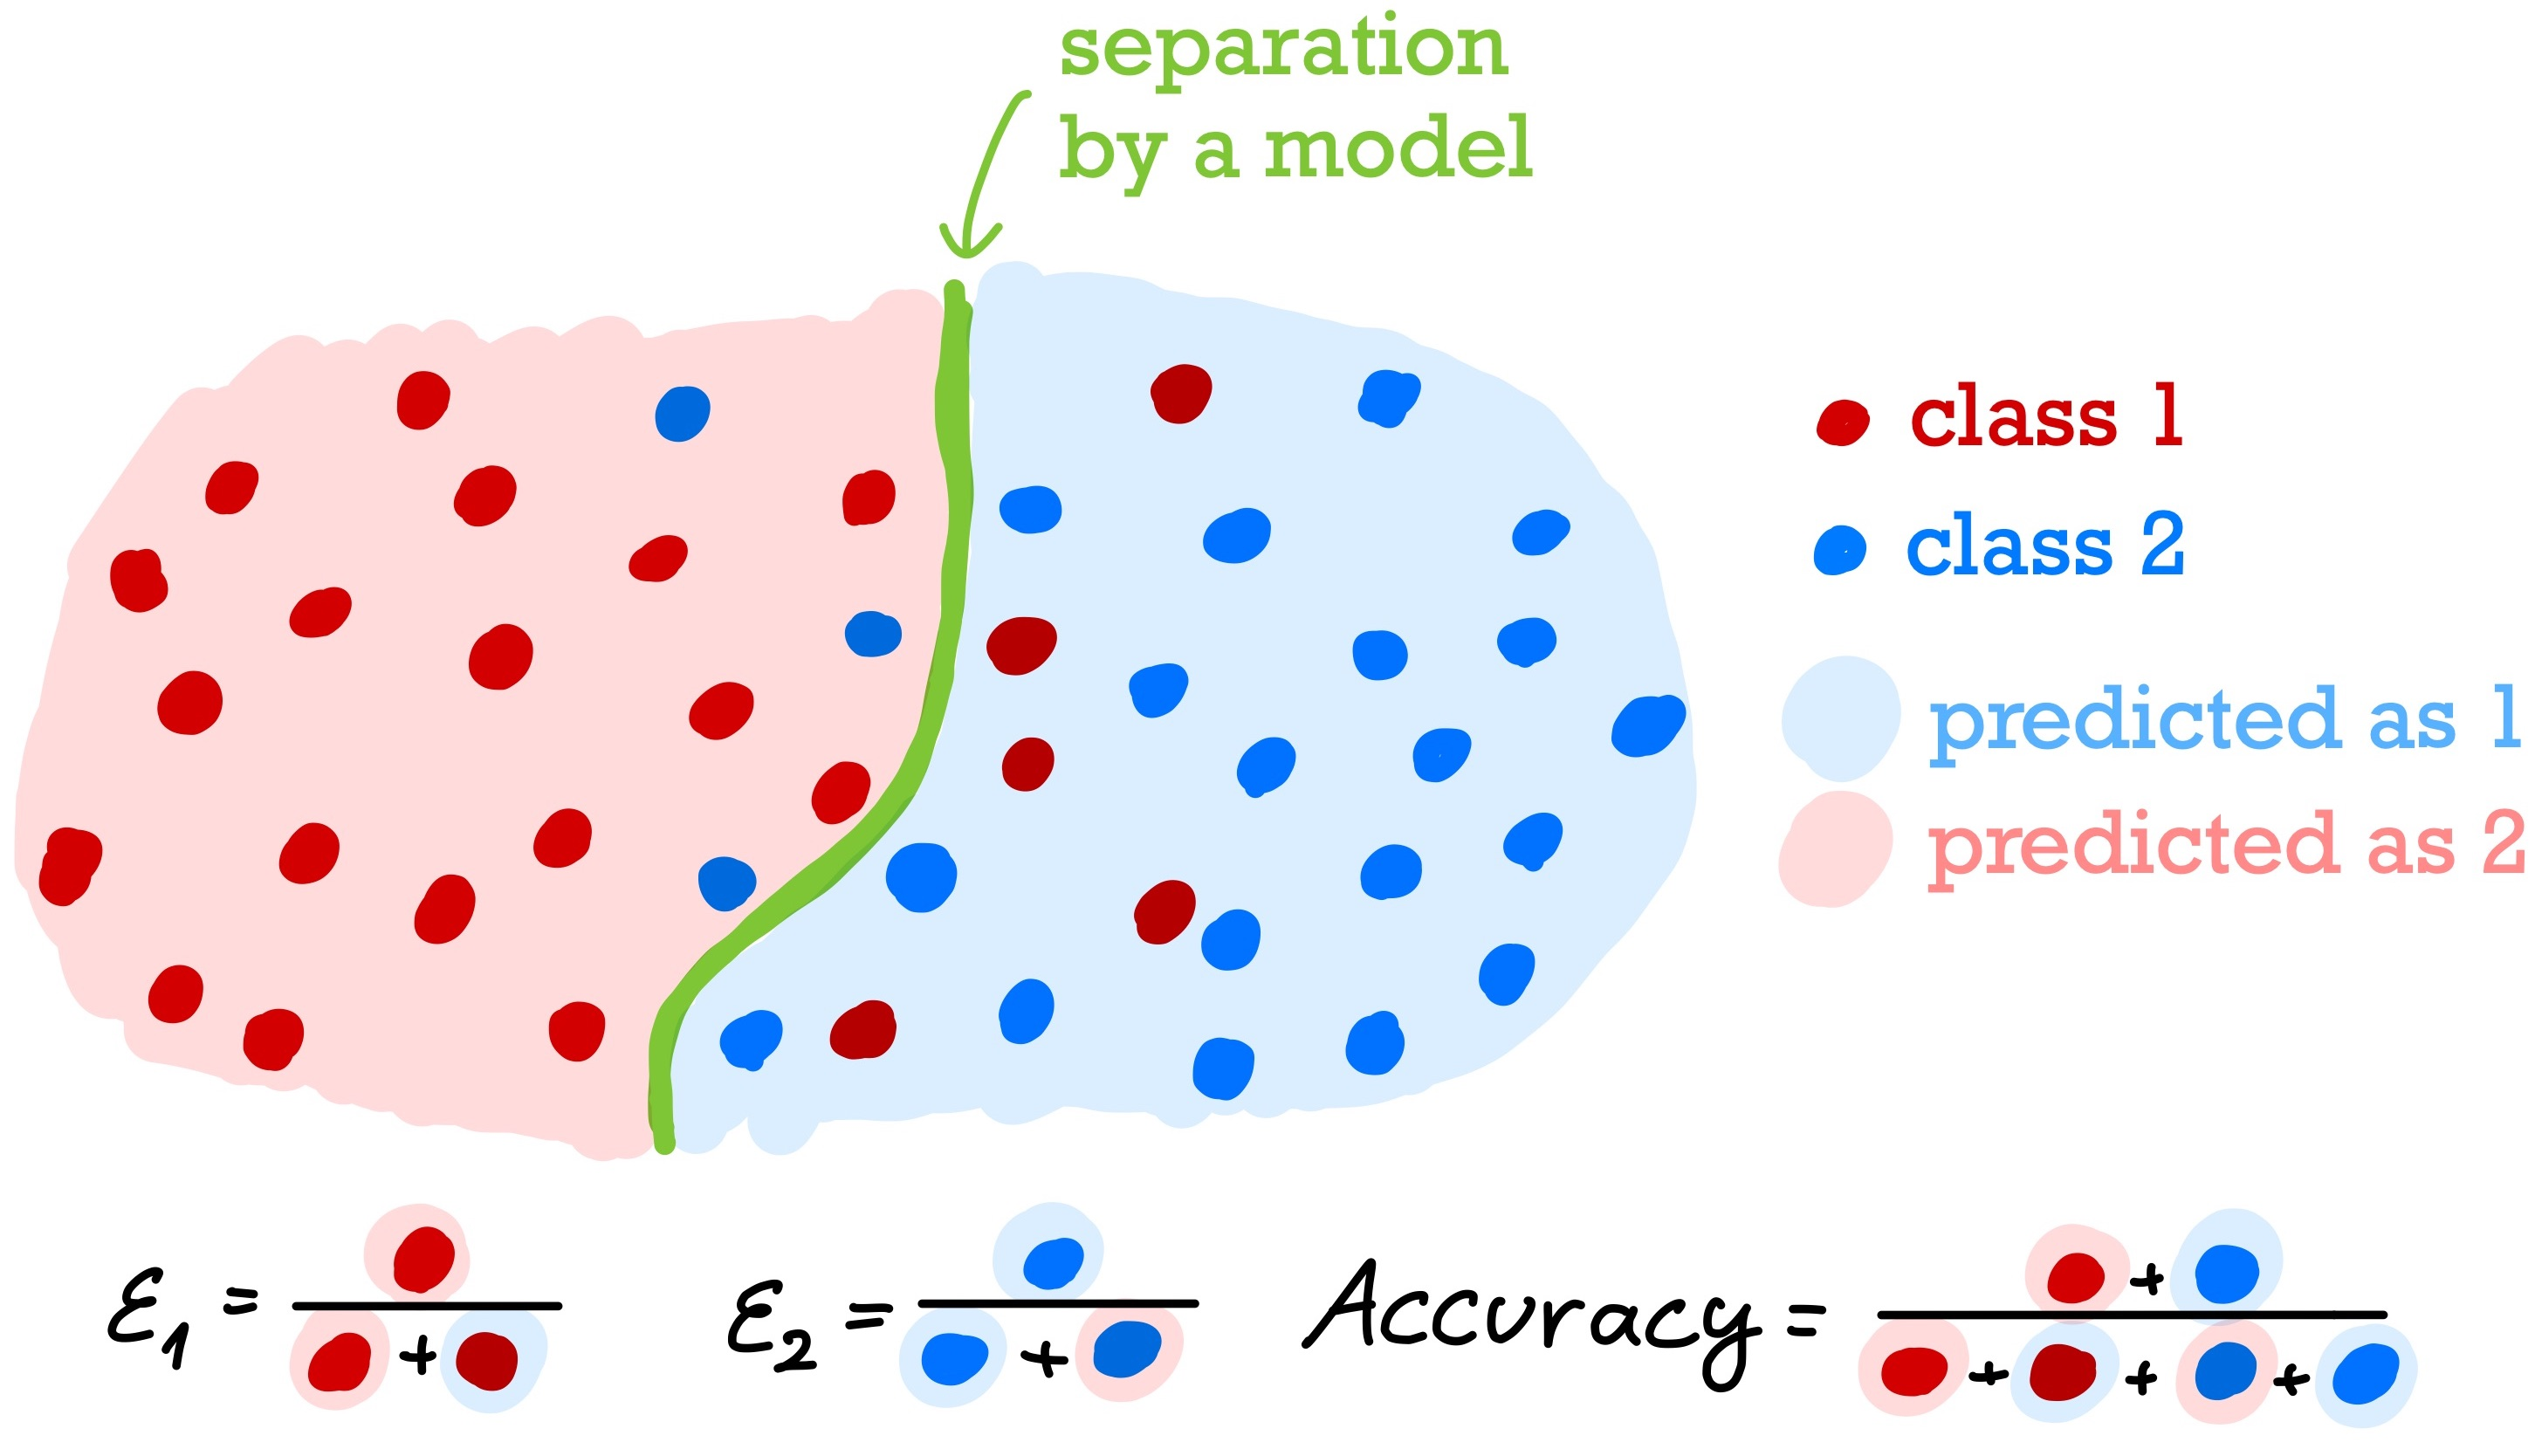
\includegraphics[width=1\linewidth]{src/img/metrics.jpg}
    \caption{Visualization of the metrics. Red dots correspond to class 1, and blue dots to class 2. The model is represented by a green line that separates the two classes. Red highlighted dots were tagged by the model as class 1, and blue highlighted dots as class 2. In formulas at the bottom, the highlighted dots represent the number of total dots with attributes given by the color and highlight.}
    \label{fig:metrics}
\end{figure}

We can now define the following metrics with a \emph{fixed threshold}:
\begin{description}
    \item[Accuracy] is the fraction of correctly classified events
    \begin{equation}
        \label{eq:accuracy}
        \text{Accuracy} = \frac{T_0 + T_1}{T_0 + T_1 + F_0 + F_1}.
    \end{equation}
    Or generally a probability of correct classification.
    \item[Efficiency] $\epsilon_i$ of class $i$ is the fraction of correctly identifying the class $i$ ($j$ is the other class)
    \begin{equation}
        \label{eq:efficiency}
        \epsilon_i = \frac{T_i}{T_i + F_j}.
    \end{equation}
    This metric has more terms if $i = 1$: \emph{true positive rate} (TPR) sensitivity, recall, hit rate, probability of detection...
    \item[Rejection] $\epsilon^{-1}_i$ of class $i$ is the inverse of fraction of correctly identifying the class $i$ ($j$ is the other class)
    \begin{equation}
        \label{eq:rejection}
        \epsilon^{-1}_i = \frac{1}{\epsilon_i} = \frac{T_i + F_j}{T_i}.
    \end{equation}
    \item[False Rate] $\varphi_i$ of class $i$ is the fraction of incorrectly identifying the class $i$ ($j$ is the other class)
    \begin{equation}
        \label{eq:false_rate}
        \varphi_i = \frac{F_i}{T_j + F_i}
    \end{equation}
    This metric has more terms if $i = 1$: \emph{false positive rate} (FPR), fall-out, probability of false alarm...
    \item[Confusion Matrix] (CM) is a plot where on the x-axis are the predicted classes, and on the y-axis are the true classes. 
    The CM is a good way to visualize the performance of the model. 
    The diagonal represents the efficiencies of a given class and the off-diagonal represents the false rates of the given class.
\end{description}

Following metrics are defined with a \emph{variable threshold}:
\begin{description}
    \item [ROC] (Receiver Operating Characteristic) curve is the plot of the efficiency $\epsilon_1$ against the false rate $\varphi_1$ for different thresholds. 
    It is good to note that there is no point in switching the classes since the ROC curve would reflect wrt—the diagonal. 
    \item[AUC] is the Area Under the ROC Curve, a simple integration of the ROC curve.
    \item[Rejection at Efficiency] $\epsilon^{-1}_i @_x \epsilon_j$ is the rejection of the one class $i$ at a given efficiency $x$ of the second class $j$ with an adjusted threshold.
\end{description}


\section{Fully Connected Network}
\label{sec:fc}
\begin{figure}[htb]
    \centering
    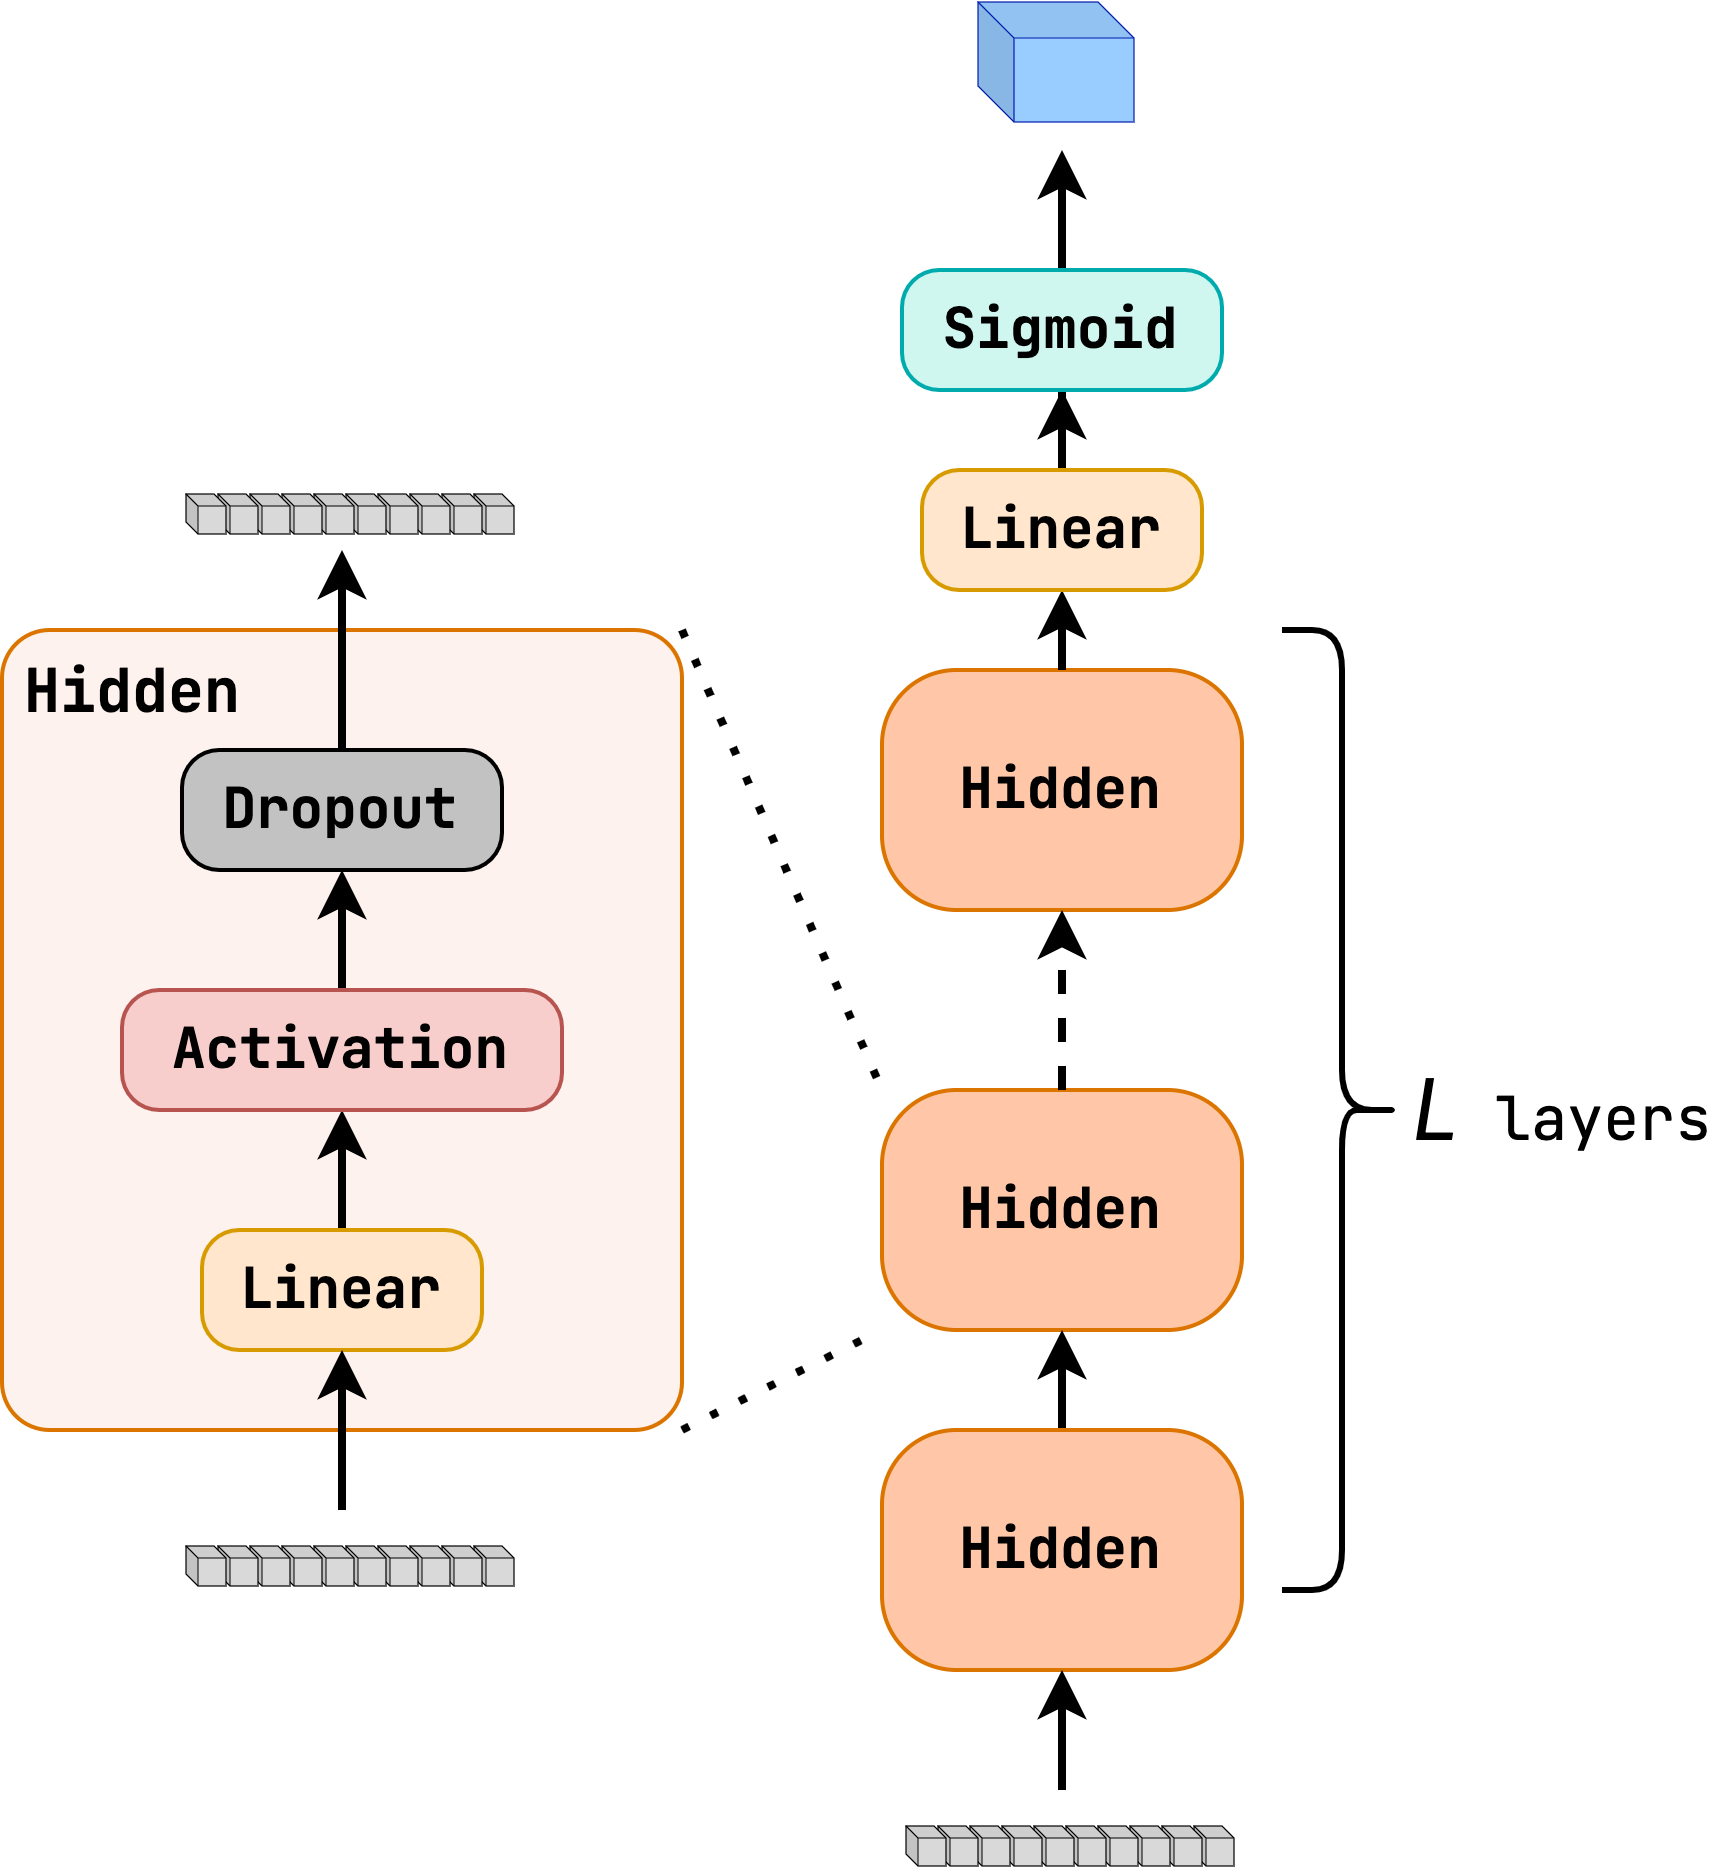
\includegraphics[width=0.6\linewidth]{src/diagrams/fc.png}
    \caption{Diagram of the Fully Connected Network.}
    \label{fig:fc}
\end{figure}

\emph{Fully Connected Network} (FC) \cite{mlp} is the most straightforward neural network, where all the neurons in one layer are connected to all the neurons in the next layer and previous layers.
It is the same as \mlp \cite{mlp}, but instead of $\tanh$ activation, we use newer activation functions described in section \ref{sec:activations}.

The input is a vector $\pmb{x}^{(0)} \in \mathbb{R}^{n_0}$ (input layer) and the output is a vector $\pmb{o} \equiv \pmb{x}^{(L + 1)} \in \mathbb{R}^{n_{L+1}}$ (output layer), where $n_{L+1}$ is the number of classes.
Between input and output layers there are $L$ hidden layers $\pmb{x}^{(l)} \in \mathbb{R}^{n_{l}}$, where $n_{l}$ is the number of neurons in the layer, i.e. \emph{layer size}.
The output of the $l$-th layer is calculated as
\begin{equation}
    \label{eq:hidden}
    \pmb{x}^{(l + 1)} = f(\pmb{W}^{(l)} \pmb{x}^{(l)} + \pmb{b}^{(l)}),
\end{equation}
where $f$ is the activation function, $\pmb{W}^{(l)} \in \mathbb{R}^{n_{l} \times n_{l-1}}$ is the weight matrix (trainable parameters), and $\pmb{b}^{(l)} \in \mathbb{R}^{n_{l}}$ is the bias vector (trainable parameters).
On the last layer, the softmax or sigmoid activation function is used. 
After each layer, we apply the dropout.
A diagram of the \fc is shown in \cref{fig:fc}.
\texttt{Linear} corresponds to the matrix multiplication and bias addition, and \texttt{Hidden} to the sequential application of the \texttt{Linear} layer \texttt{Activation} and \texttt{Dropout}.
At the output, there is no dropout.

A more artistic diagram of the \fc is shown in \cref{fig:fc2}.
\begin{figure}[htb]
    \centering
    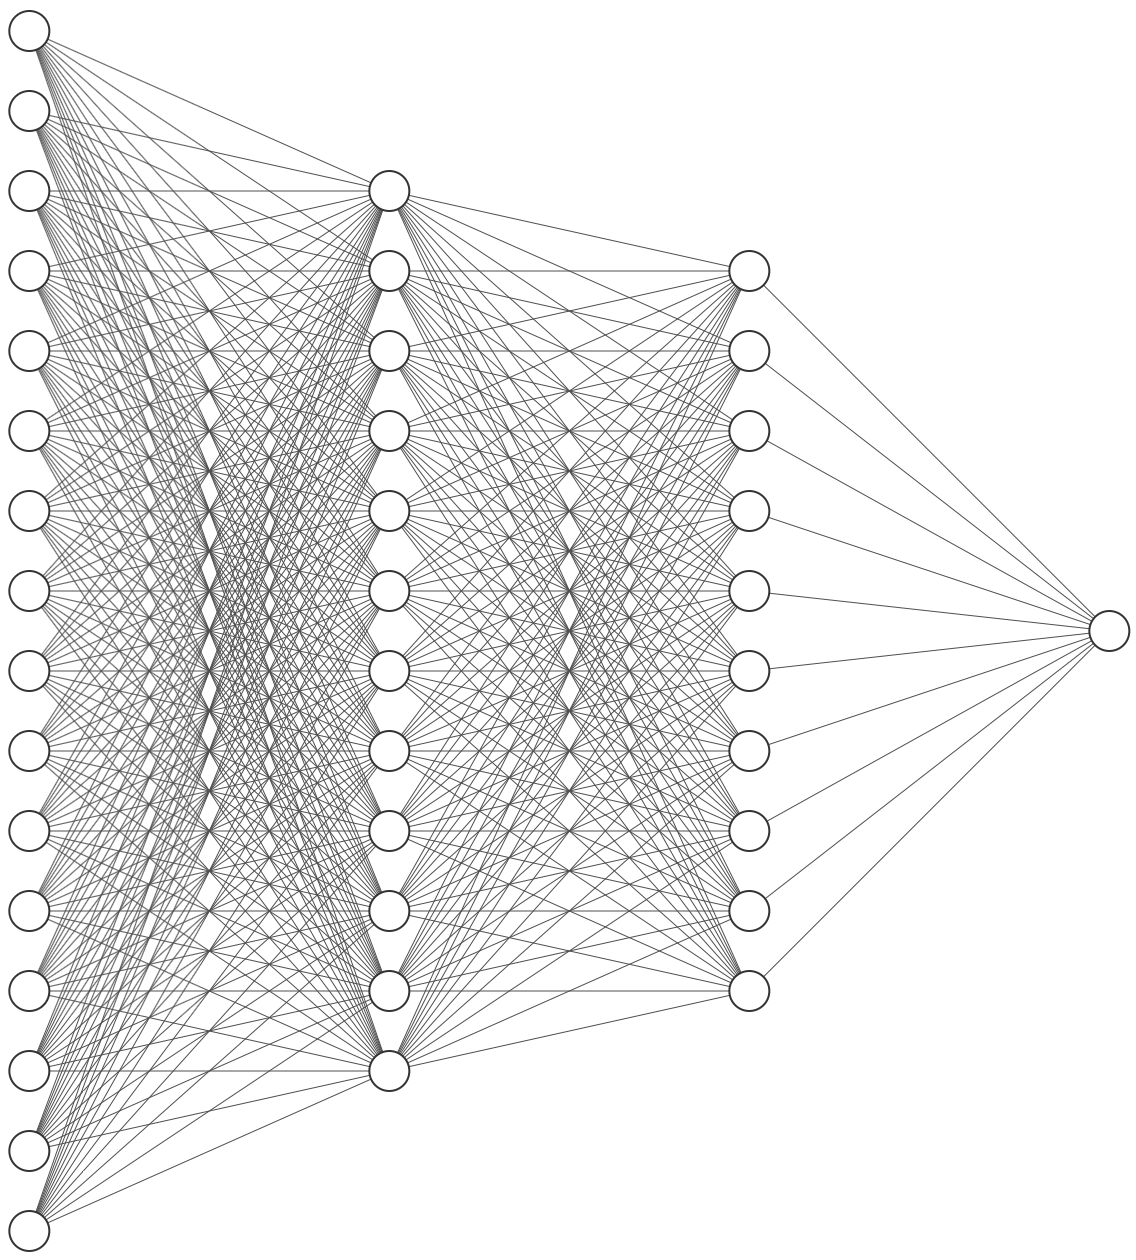
\includegraphics[width=0.5\linewidth]{src/img/fc.png}
    \caption[Artistic diagram of the Fully Connected Network. Each node is a \emph{neuron} corresponding to a number in a vector $\pmb{x}^{(l)}$, and each edge is a weight corresponding to a number in matrix $\pmb{W}^{(l)}$.]{Artistic diagram of the Fully Connected Network\footnotemark. Each node is a \emph{neuron} corresponding to a number in a vector $\pmb{x}^{(l)}$, and each edge is a weight corresponding to a number in matrix $\pmb{W}^{(l)}$.}
    \label{fig:fc2}
\end{figure}
\footnotetext{\url{https://github.com/ashishpatel26/Tools-to-Design-or-Visualize-Architecture-of-Neural-Network}.}

In our case, the input vector $\pmb{x}^{(0)}$ are \emph{high-level jet variables} and the output vector is just one number $o$, which is the probability of the jet being a quark (1) or gluon (0).
This type of network allows us to utilize the reconstructed jet, whose properties are given by the \PFOs.
However, it \textbf{cannot utilize} the information about the \textbf{PFOs} themselves.

\section{Highway Network}

\label{sec:highway}
\begin{figure}[htb]
    \centering
    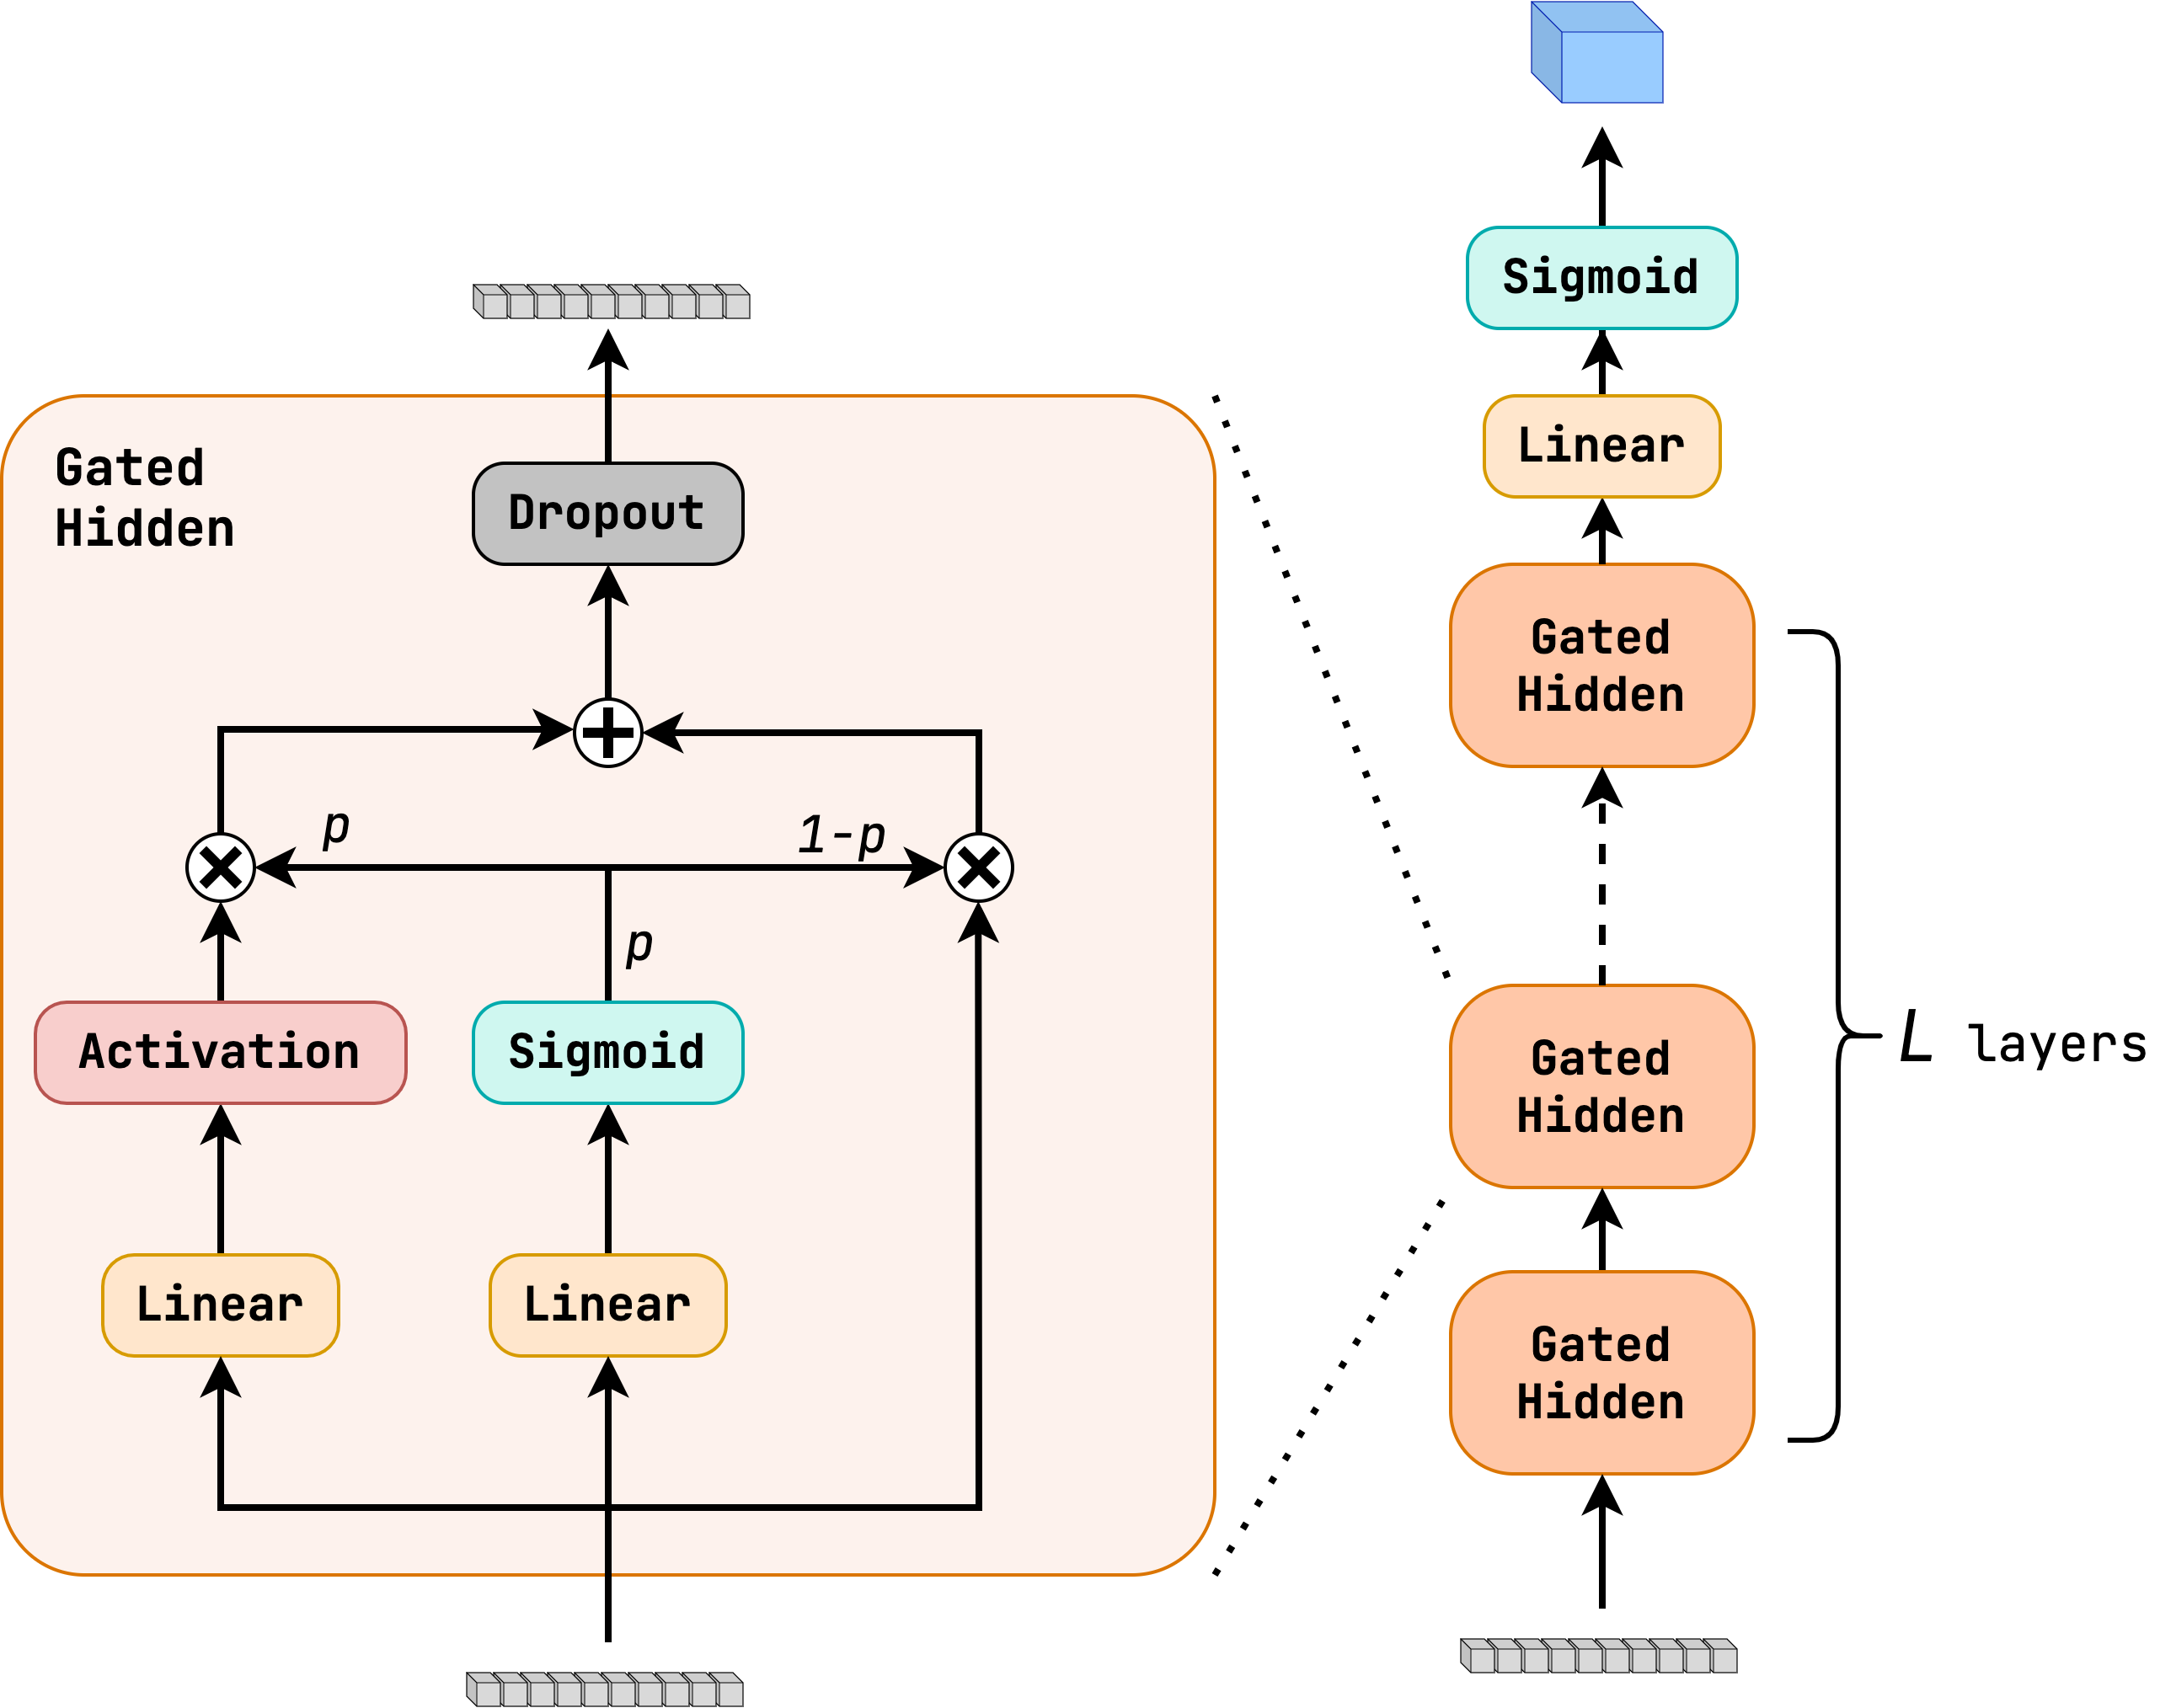
\includegraphics[width=0.8\linewidth]{src/diagrams/highway.png}
    \caption{Diagram of the Highway Network.}
    \label{fig:highway}
\end{figure}

\emph{Highway Network} \cite{highway} is an extension of the \fc network, that introduces a \emph{gate} to the network.
The gate is a \emph{bypass} that allows the output of one layer to pass through the next layer without any modification.
Another term for the bypass is a \emph{residual connection}.
The gate is a \emph{learnable} function controlling the amount of data bypassing the layer.
It multiplies the output of the hidden layer by a probability $p$ and adds the input of the layer multiplied by $1 - p$
\begin{equation}
    \pmb{x}^{(l + 1)} = p f(\pmb{W}^{(l)} \pmb{x}^{(l)} + \pmb{b}^{(l)}) + (1 - p) \pmb{x}^{(l)} . 
\end{equation}

The trick is estimating the probability $p$ of using the newly calculated output rather than the input.
It is calculated from the input vector $\pmb{x}^{(l)}$ and another weight matrix $\pmb{W}^{(l)}_{\text{g}}$ (and bias $\pmb{b}^{(l)}_{\text{g}}$) followed by a sigmoid activation function, whose output is a probability.
\begin{equation}
    \pmb{p}^{(l)} = \sigma(\pmb{W}^{(l)}_{\text{g}} \pmb{x}^{(l)} + \pmb{b}^{(l)}_{\text{g}}),
\end{equation}
where the probabilities are calculated for each element of the vector $\pmb{x}^{(l)}$ separately and are different for each layer.
The output of the \highway layer is then calculated as
\begin{equation}
    \pmb{x}^{(l + 1)} = \pmb{p}^{(l)} \cdot f(\pmb{W}^{(l)} \pmb{x}^{(l)} + \pmb{b}^{(l)}) + (1 - \pmb{p}^{(l)}) \cdot \pmb{x}^{(l)} ,
\end{equation}
where $\cdot$ is the element-wise multiplication.
If we put it all together, one layer of \highway can be written as
\begin{equation}
    \pmb{x}^{(l + 1)} = \sigma(\pmb{W}^{(l)}_{\text{g}} \pmb{x}^{(l)} + \pmb{b}^{(l)}_{\text{g}}) \cdot f(\pmb{W}^{(l)} \pmb{x}^{(l)} + \pmb{b}^{(l)}) + (1 - \sigma(\pmb{W}^{(l)}_{\text{g}} \pmb{x}^{(l)} + \pmb{b}^{(l)}_{\text{g}})) \cdot \pmb{x}^{(l)}.
\end{equation}
Everything else (output, dropout, activation function) is the same as in the \fc network.
The diagram of the \highway is shown in \cref{fig:highway}.

\highway uses the same input as the \fc network, i.e. the \emph{high-level jet variables}.
The only advantage of the \highway network is that it is \textbf{more stable} when training the network with many layers.

\section{Particle Flow and Energy Flow Network}
\label{sec:pfn_efn}

\begin{figure}[htb]
    \centering
    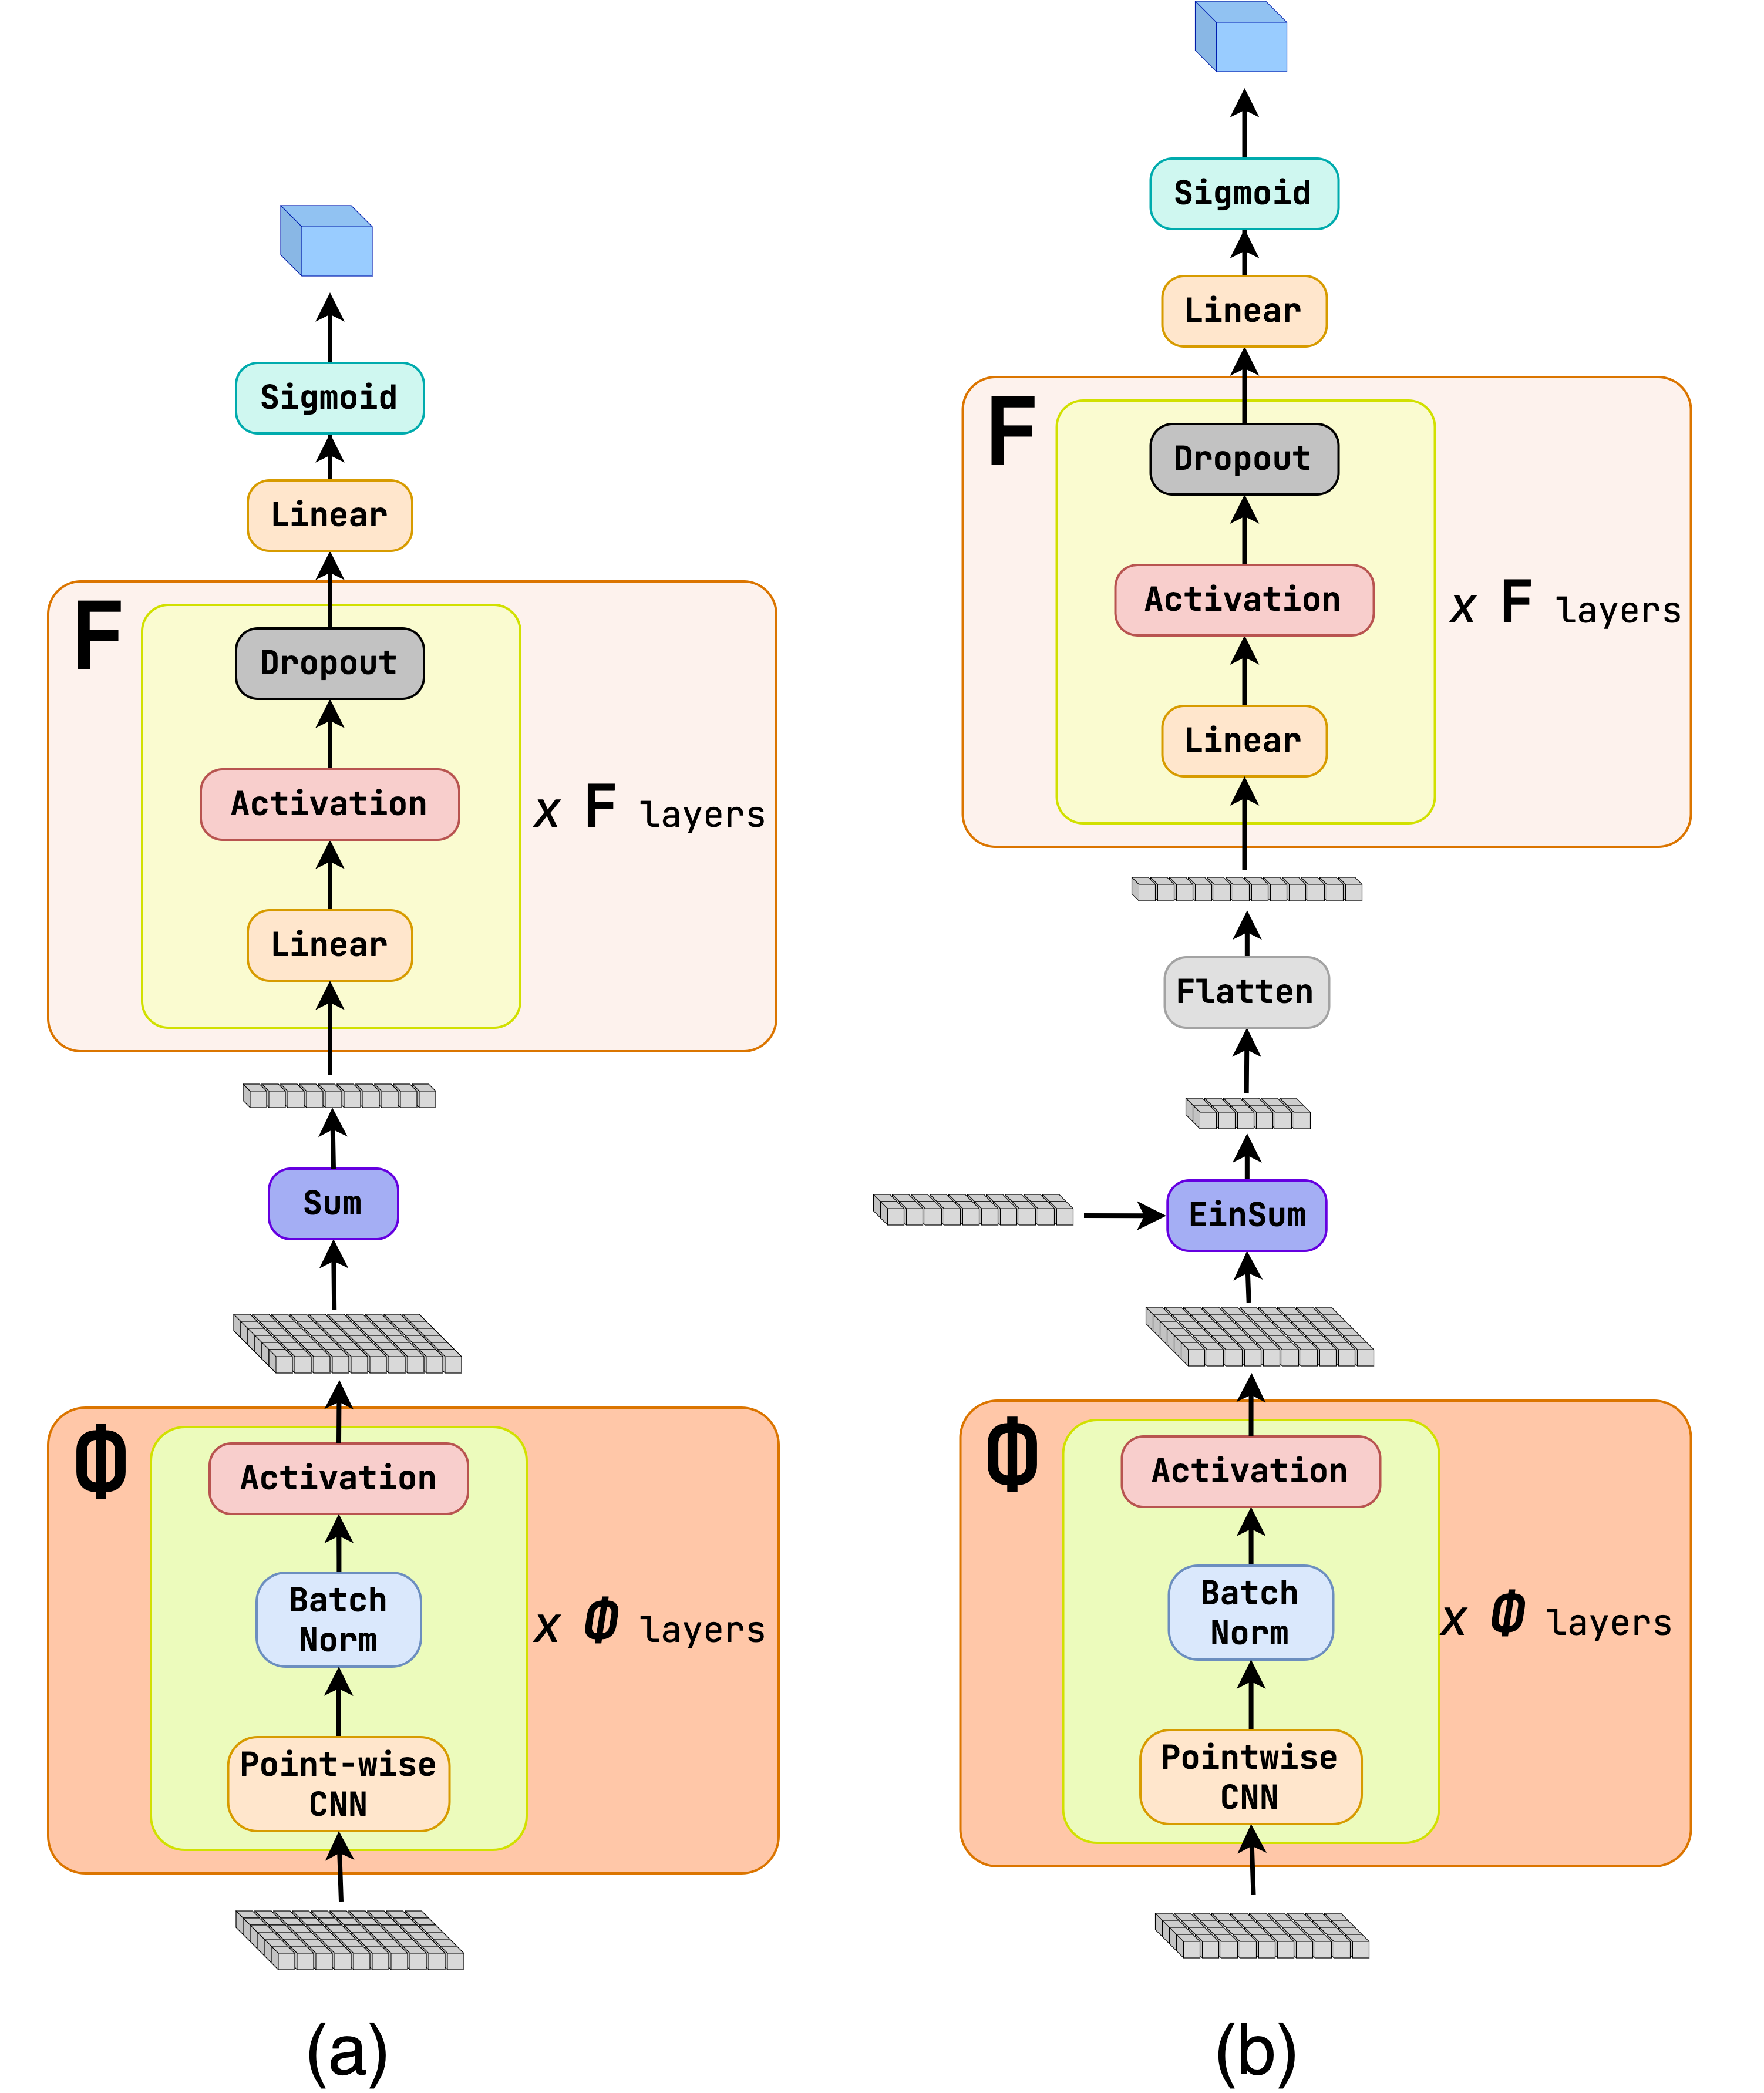
\includegraphics[width=0.7\textwidth]{src/diagrams/pfn_efn.png}
    \caption{Diagram of PFN (a) and EFN (b). The \texttt{Einsum} layer corresponds to \texttt{tf.einsum} function and Point-wise CNN to \texttt{tf.keras.layers.Conv1D(filters=layer\_size, kernel\_size=1)}.}
    \label{fig:pfn_efn}
\end{figure}

\emph{Particle Flow Network} (PFN) and \emph{Energy Flow Network} (EFN) \cite{efn} are two networks that are designed to utilize the information about the \PFOs.
They are developed specifically for \HEP, using the theory of \emph{Deep Sets} \cite{deep_set}.

The general idea is in three steps:
\begin{enumerate}
    \item \emph{Per \PFO Mapping}   
    \item \emph{Summing over \PFOs} 
    \item \emph{Constructing Observable}
\end{enumerate}

In the case of \PFN, this can be expressed in the form 
\begin{equation}
    \label{eq:pfn}
  \mathcal{O_{\text{PFN}}} = F\left(\sum_{i=1}^N \Phi(\pmb{z}_i, \pmb{\varphi}_i )\right), 
\end{equation}  
where the function $F$ constructs the \emph{observable} $\mathcal{O}$, $\Phi$ is the \emph{per \PFO mapping}, $\pmb{z}_i$ is a vector of \PFO energy properties ($\pT$ or $E$) and $\pmb{\varphi}_i$ is a vector of \PFO angular properties ($\eta$, $\theta$, $\phi$).

\EFN is similar to \PFN but is specifically designed to be IRC safe (see \cref{def:IRC})
\begin{equation}
    \label{eq:efn}
    \mathcal{O_{\text{EFN}}} = F\left(\sum_{i=1}^N \pmb{z}_i \Phi(\pmb{\varphi}_i )\right).
\end{equation}
The mapping $\Phi$ is the same as in \PFN, but the \PFO energy properties are \emph{not used}. 
The linearity in $\pmb{z}_i$ satisfies the IRC conditions.

To construct the mapping $\Phi$ and the function $F$, the authors \cite{efn} use the \emph{Universal Approximation Theorem} \cite{universal_app_thm} discussed in \cref{sec:activations} to make the argument that \fc is sufficient to approximate any function.
For the $F$ function, we use the architecture of the \fc network with \texttt{$F$\_layers} a number of \texttt{hidden} layers, but for the $\Phi$ function, we use the \pointCNN \cite{pointCNN}, which is a slight improvement over the \fc network still agreeing with the (\ref{eq:pfn}) or (\ref{eq:efn}).
The \pointCNN is followed by \emph{batch normalization} and activation to form a block that is repeated \texttt{$\Phi$\_layer} times.

In the case of \EFN, the summation over the \PFOs is a matrix multiplication over the \PFO index. 
The output is a matrix (because both $\pmb{z_i}$ and $\pmb{\varphi_i}$ are matrices) which is then flattened to a vector.\footnote{This is done using the \texttt{tf.einsum} function, hence the name in \cref{fig:pfn_efn}, followed by a \texttt{tf.reshape}.}
This is not the case in the original paper, but this modification's performance is much better, still satisfying the IRC conditions and the form of (\ref{eq:efn}).
The accompanying diagram of both \PFN and \EFN is shown in \cref{fig:pfn_efn}.


The main advantage of \PFN and \EFN is that they are designed to use the information about the \PFOs, which is not the case for the \fc or \highway.
On top of that, \EFN is IRC-safe, which is crucial in the case of \HEP.
In the case of model performance, this advantage can be seen when comparing the performance of data from different physics simulation frameworks \cite{top_tag}.
However, the biggest downside of \PFN and \EFN is that they \textbf{do not allow} the \textbf{PFOs to communicate} and share information.

\section{Transformer}
\label{sec:transformer}

\begin{figure}[htb]
    \centering
    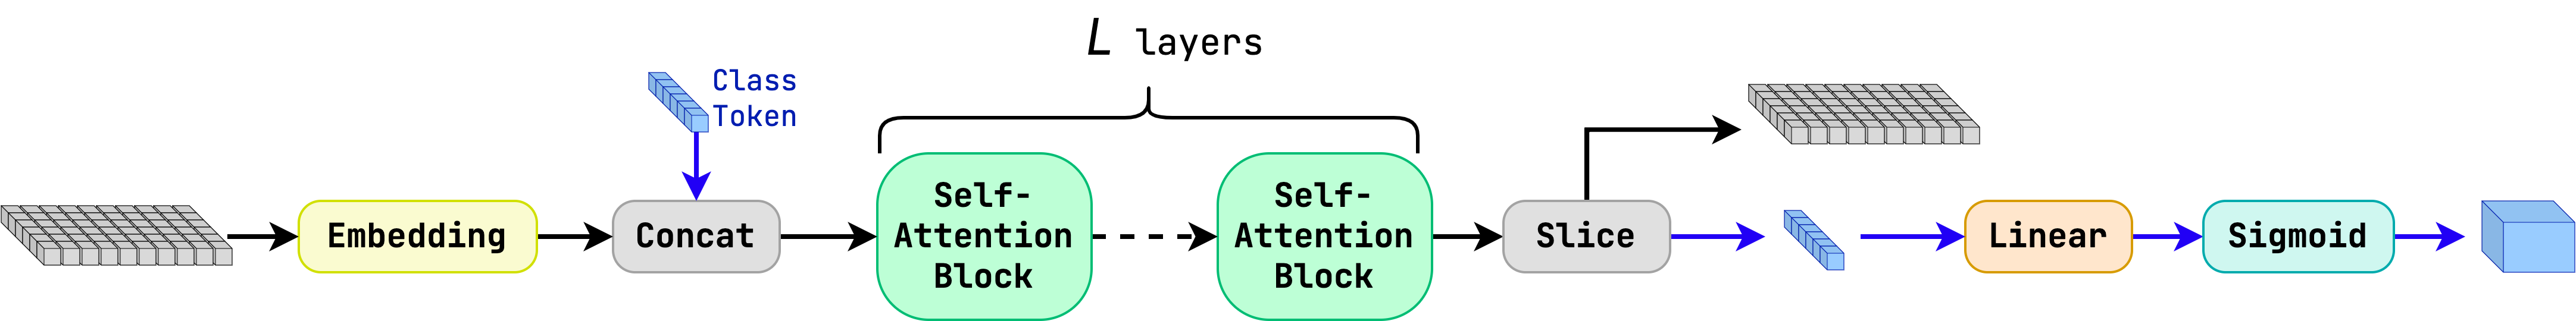
\includegraphics[width=1.\linewidth]{src/diagrams/transformer.png}
    \caption{Diagram of the Transformer. The \emph{Class Token} is represented as a blue row of boxes. Operations concerning the \emph{Class Token} are traced with a blue arrow.}
    \label{fig:trans}
\end{figure}

\begin{figure}[htb]
    \centering
    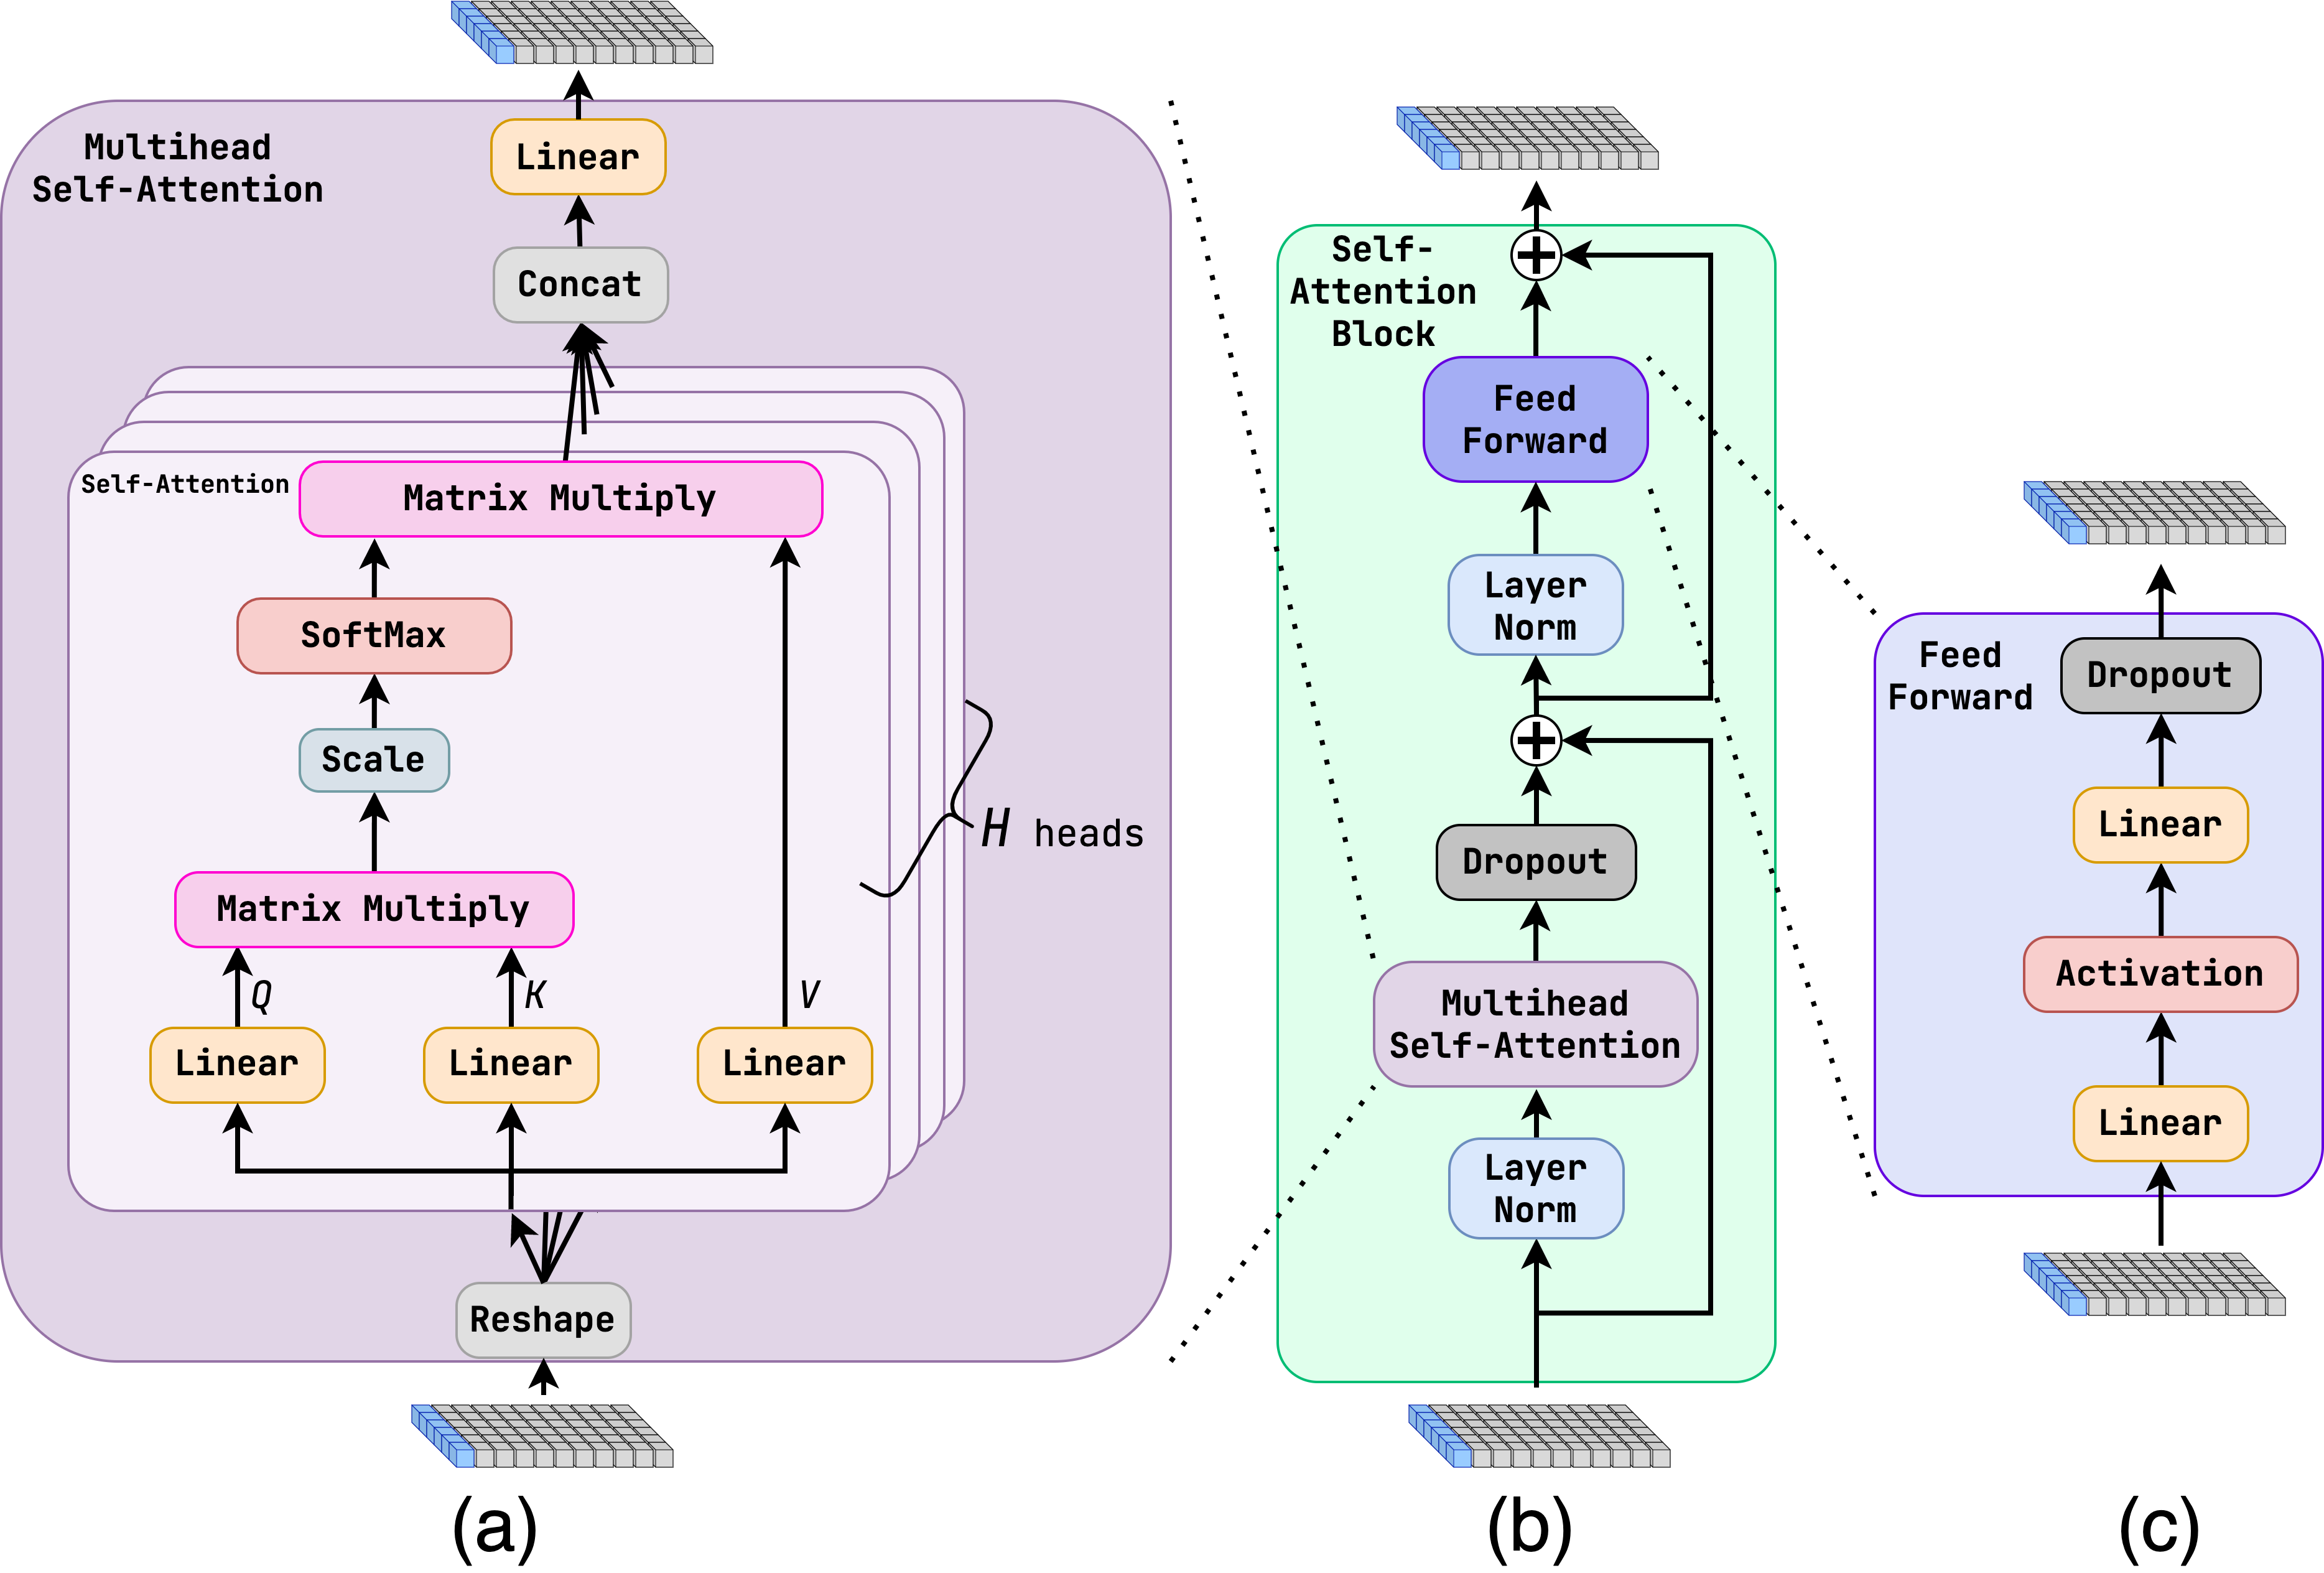
\includegraphics[width=0.9\linewidth]{src/diagrams/transformer_layers.png}
    \caption{Diagram of the Transformer layers. (b) is the \emph{Self-Attention Block}, with the main components being the \emph{Multihead Self-Attention} (a) and the \emph{Feed Forward Network} (c). The \emph{Class Token} is represented as a blue row of boxes.}
    \label{fig:trans_layers}
\end{figure}

\emph{Transformer} \cite{att_is_all} is a network designed to learn from set data with fixed \emph{embedding} dimension.
It is based on the \emph{Attention} mechanism, which is a core component of \trans network, allowing the elements of the set to \textbf{communicate} with each other.
The overall structure of the original \trans consists of \emph{Encoder} and \emph{Decoder} blocks, but in our use case, we only use the Encoder part, which is shown in \cref{fig:trans}.
The Encoder part is supposed to form a \emph{representation} of the input data based on the task.
On the other hand, the Decoder part reconstructs some output data from the internal representation of the Encoder part.
To give a more concrete example, imagine a translation between languages such as Czech and Slovak.
The Encoder represents what the input Czech sentence is trying to say, i.e., the abstract information, and the Decoder reconstructs the Slovak sentence from the internal representation of the Encoder.
As stated, we are only interested in forming the internal representation of the input data, so we only use the Encoder part of the \trans, accompanied by information extraction from the internal representation.

The whole Transformer starts with an \emph{embedding} of the input set, expanding the dimension of the input data to the \texttt{embed\_dim}, allowing the model to learn more complex representations.
The embedding layer is just a \fc layer with \texttt{embed\_dim} neurons and multiple hidden layers, as shown in \cref{fig:embed} (a).
After which come the \SA Blocks (\cref{sec:SA_block}), whose core components are the \MHSA (\cref{sec:mhsa}) and \FFN (\cref{sec:ffn}).
The \emph{class extraction} is done using the \emph{Class Token} (\cref{sec:class_extract}).

The \trans architecture provides a way for \textbf{PFOs to communicate} and exchange valuable information, creating a complete representation of the jet (input data).
Despite its complexity, the \trans provides an immense advantage over the \PFN and \EFN, which is the ability to \textbf{learn long-range dependencies} in the input data.

\subsection{Multihead Self-Attention}
\label{sec:mhsa}
The input of the \emph{Multihead Self-Attention} layer is a set of $N$ vectors with dimension \texttt{embed\_dim}, denoted as $C$, with overall batched shape $B \times N \times C$, where $B$ is the batch size.
Every input vector creates 3 'signs':
\begin{enumerate}
    \item \textbf{Queries} $Q$ representing questions of a given vector asking each other vector in the set (for example: 'What is the highest $\pT$? in the set')
    \item \textbf{Keys} $K$ representing if the given vector has the answer to the questions of other vectors (for example: 'I have the highest $\pT$.')
    \item \textbf{Values} $V$ representing the answer to the questions of other vectors (for example: 'My $\pT$ is 100 GeV.')
\end{enumerate}
These three components are constructed from the input data. 
In the case of general Attention for $Q$, $K$, and $V$ can be the input data Attention (some other input asks the question, some additional input has the keys, and some other the values).
Self-Attention is a particular case of Attention where $Q$, $K$, and $V$ are created from the same input, i.e., the input data is asking itself the questions, and the input data is the answer to the questions.
Going further in this section, we will only focus on \SA.

The \MHSA layer is shown in \cref{fig:trans_layers} (a) for visual aid. 
$Q$, $K$, and $V$ are constructed from the same input data by the three \texttt{Linear} layers.
After, the $Q$ and $V$ are matrix-multiplied across the embedding index ($C$), resulting in a matrix of shape $B \times N \times N$.
This matrix is then scaled, and the softmax activation is applied to form a probability distribution for each vector over the set, stating how much \emph{Attention} should be paid to each vector in the set to get the answer to the asked question.
This can be expressed as 
\begin{equation}
    \label{eq:attn}
    \text{\texttt{Attention}} = \text{softmax}\left(\frac{QK^T}{\sqrt{d}}\right)
\end{equation}
resulting in a matrix of shape $B \times N \times N$.
Multiplying the \texttt{Attention} by the $V$ matrix extracts the answer, resulting in a  matrix of shape $B \times N \times C$, the same shape as the input data.

Instead of doing the Attention mechanism across the whole embedding dimension, the \trans uses multiple \emph{heads}.
Each head is a separate Attention mechanism with the head dimension $d = C / H$, where $H$ is the number of heads. 
Each head's input and output shape is $B \times N \times C/H$, constructed by reshaping the input data to $B \times H \times N \times C/H$ (the calculations across the heads are done in parallel, hence the extra dimension).
The heads are concatenated, resulting in an output of shape $B \times N \times C$.
As a result, the argument of Attention must be scaled by $\sqrt{d}$, as stated in \cref{eq:attn}.

\subsection{Feedforward Network}
\label{sec:ffn}
The \emph{Feed Forward Network} (FFN) is a simple network with two \texttt{Linear} layers with \texttt{Activation} between them.
Its primary purpose is to allow the individual vectors to learn from the data obtained from other vectors in the \MHSA layer. 
The size of the first layer is \texttt{embed\_dim} $\cdot$ \texttt{expansion}, where \texttt{expansion} is a hyperparameter.
The second layer is the \texttt{embed\_dim} size to retain the original dimension of the input data.
The dropout is applied to the output of the second layer.


\subsection{Self-Attention Block}
\label{sec:SA_block}
The \emph{Self-Attention Block} (SA Block) has a \MHSA part and a \FFN part as seen in \cref{fig:trans_layers} (b).
Before the \MHSA and \FFN part, the input data is normalized using the \LN. 
\LN computes the mean and standard deviation of the input data and normalizes it across the embedding dimension such that the mean is 0 and the standard deviation is 1.
The mean and standard deviation are learned parameters, so the \LN is a trainable layer.

The dropout layer is put after the \MHSA preventing overfitting.

Across the \MHSA and \FFN part is the \emph{residual connection}, which is a simple addition of the input data and the output of the \MHSA and \FFN part.
This forces the model to learn new information on top of what is already in the input data.

The \SA Block are stacked on each other, constructing $L$ layers, which are the heart of the \trans.

\subsection{Class Extraction}
\label{sec:class_extract}
The \trans is a general-purpose model capable of learning any representation.
To extract the class information of the whole input, we use the \emph{Class Token} \cite{bert}.
The \emph{Class Token} is a vector of trainable parameters (of the same \texttt{embed\_dim} shape as input vectors) concatenated at the beginning of the input data.
It passes through the \trans layers with the input vectors extracting and storing the class information.
At the end of \SA Blocks, the output is sliced (taking only the first vector, the \emph{Class Token}) and passed through a \texttt{Linear} layer to get the final output followed by sigmoid or softmax Activation.

\begin{figure}[htb]
    \centering
    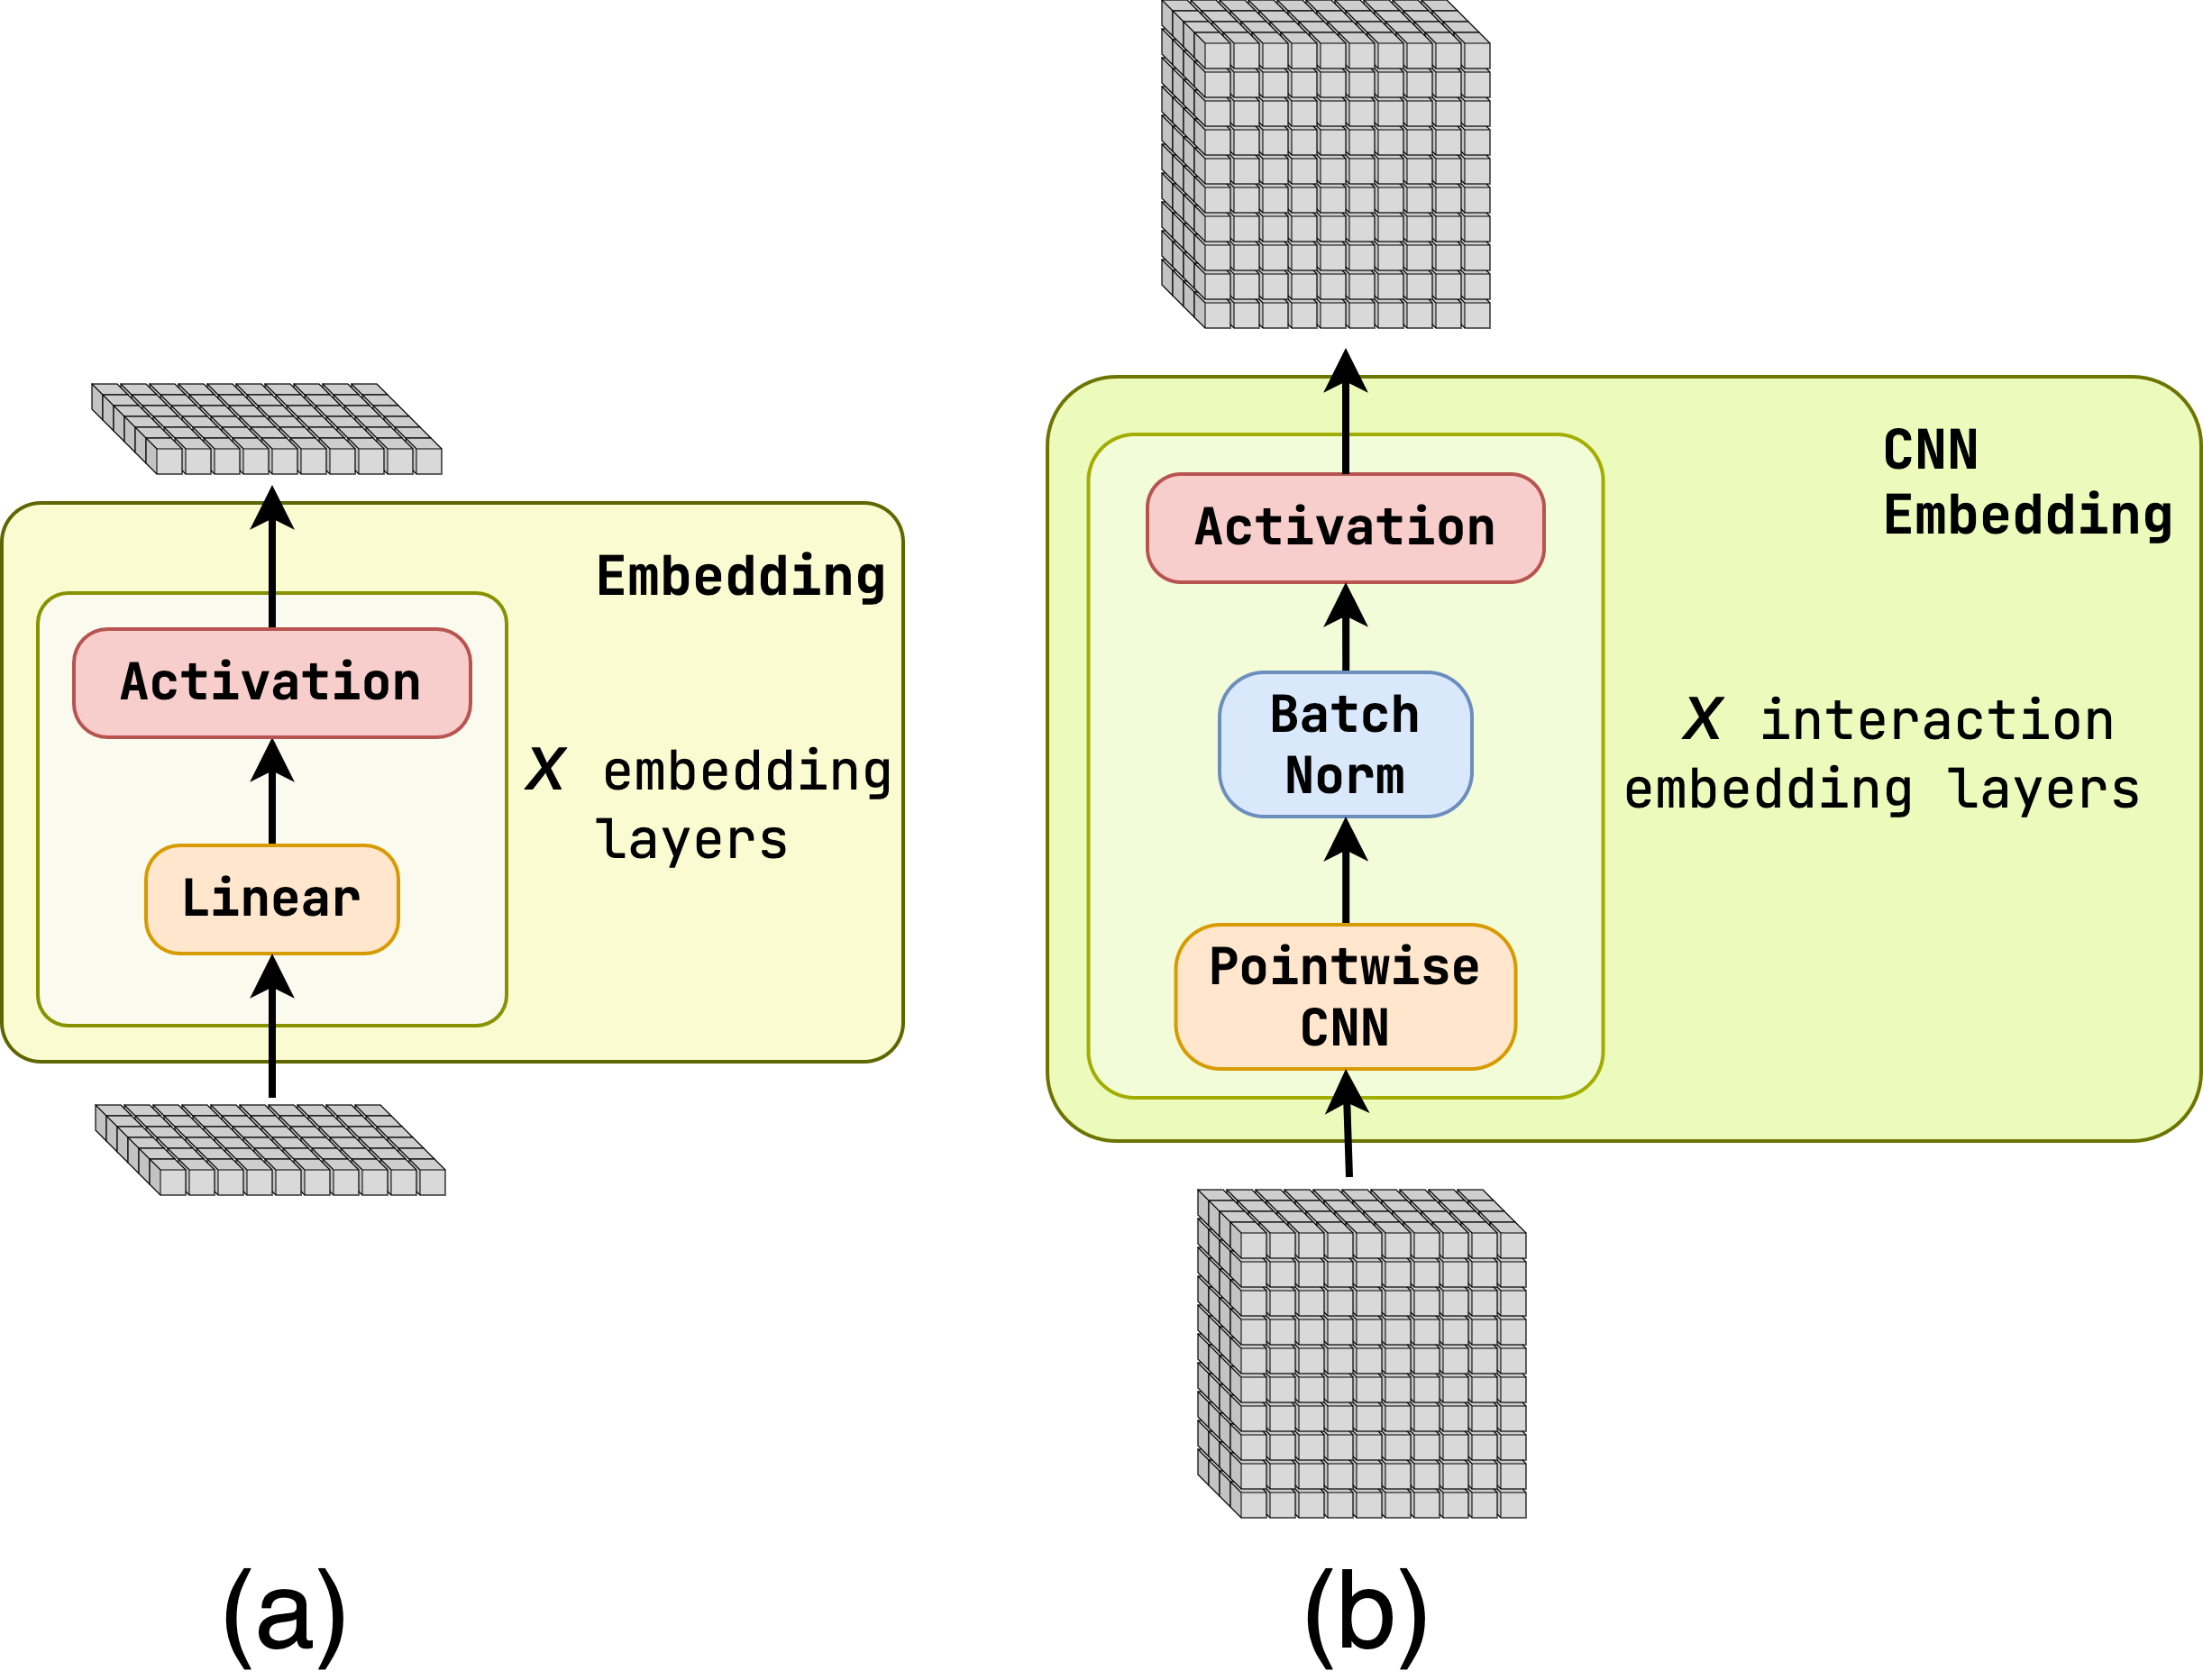
\includegraphics[width=0.7\linewidth]{src/diagrams/embedding.png}
    \caption{Embedding layers. (a) is a per-input vector embedding, and (b) is the embedding of interaction variables.}
    \label{fig:embed}
\end{figure}
\section{Particle Transformer}
\label{sec:part}
\begin{figure}[htb]
    \centering
    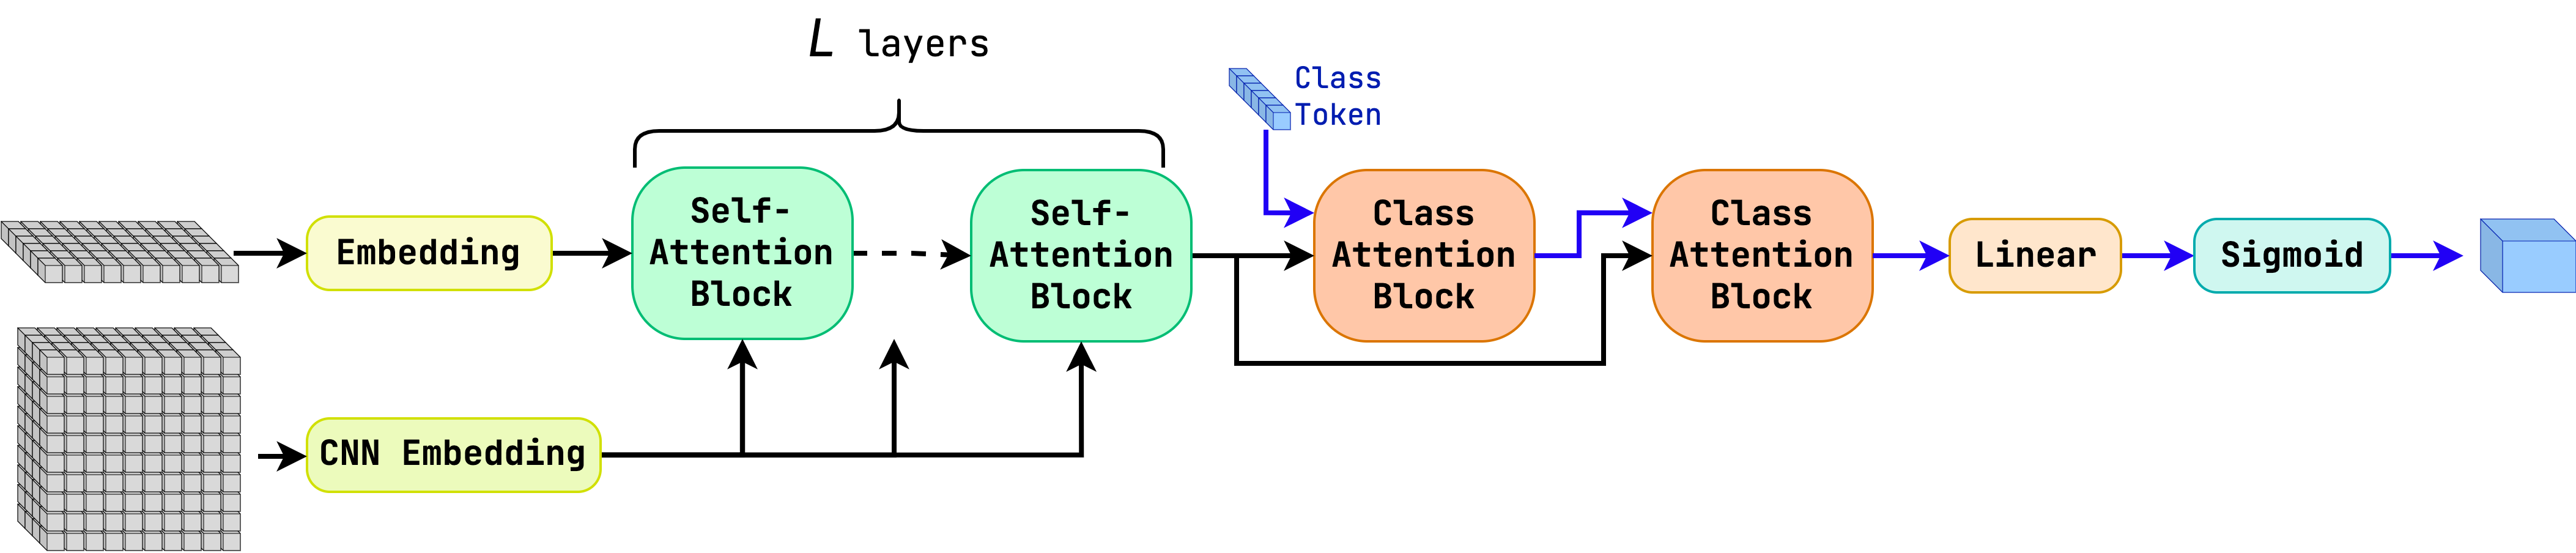
\includegraphics[width=0.9\linewidth]{src/diagrams/part.png}
    \caption{Particle Transformer architecture.}
    \label{fig:part}
\end{figure}

\begin{figure}[htb]
    \centering
    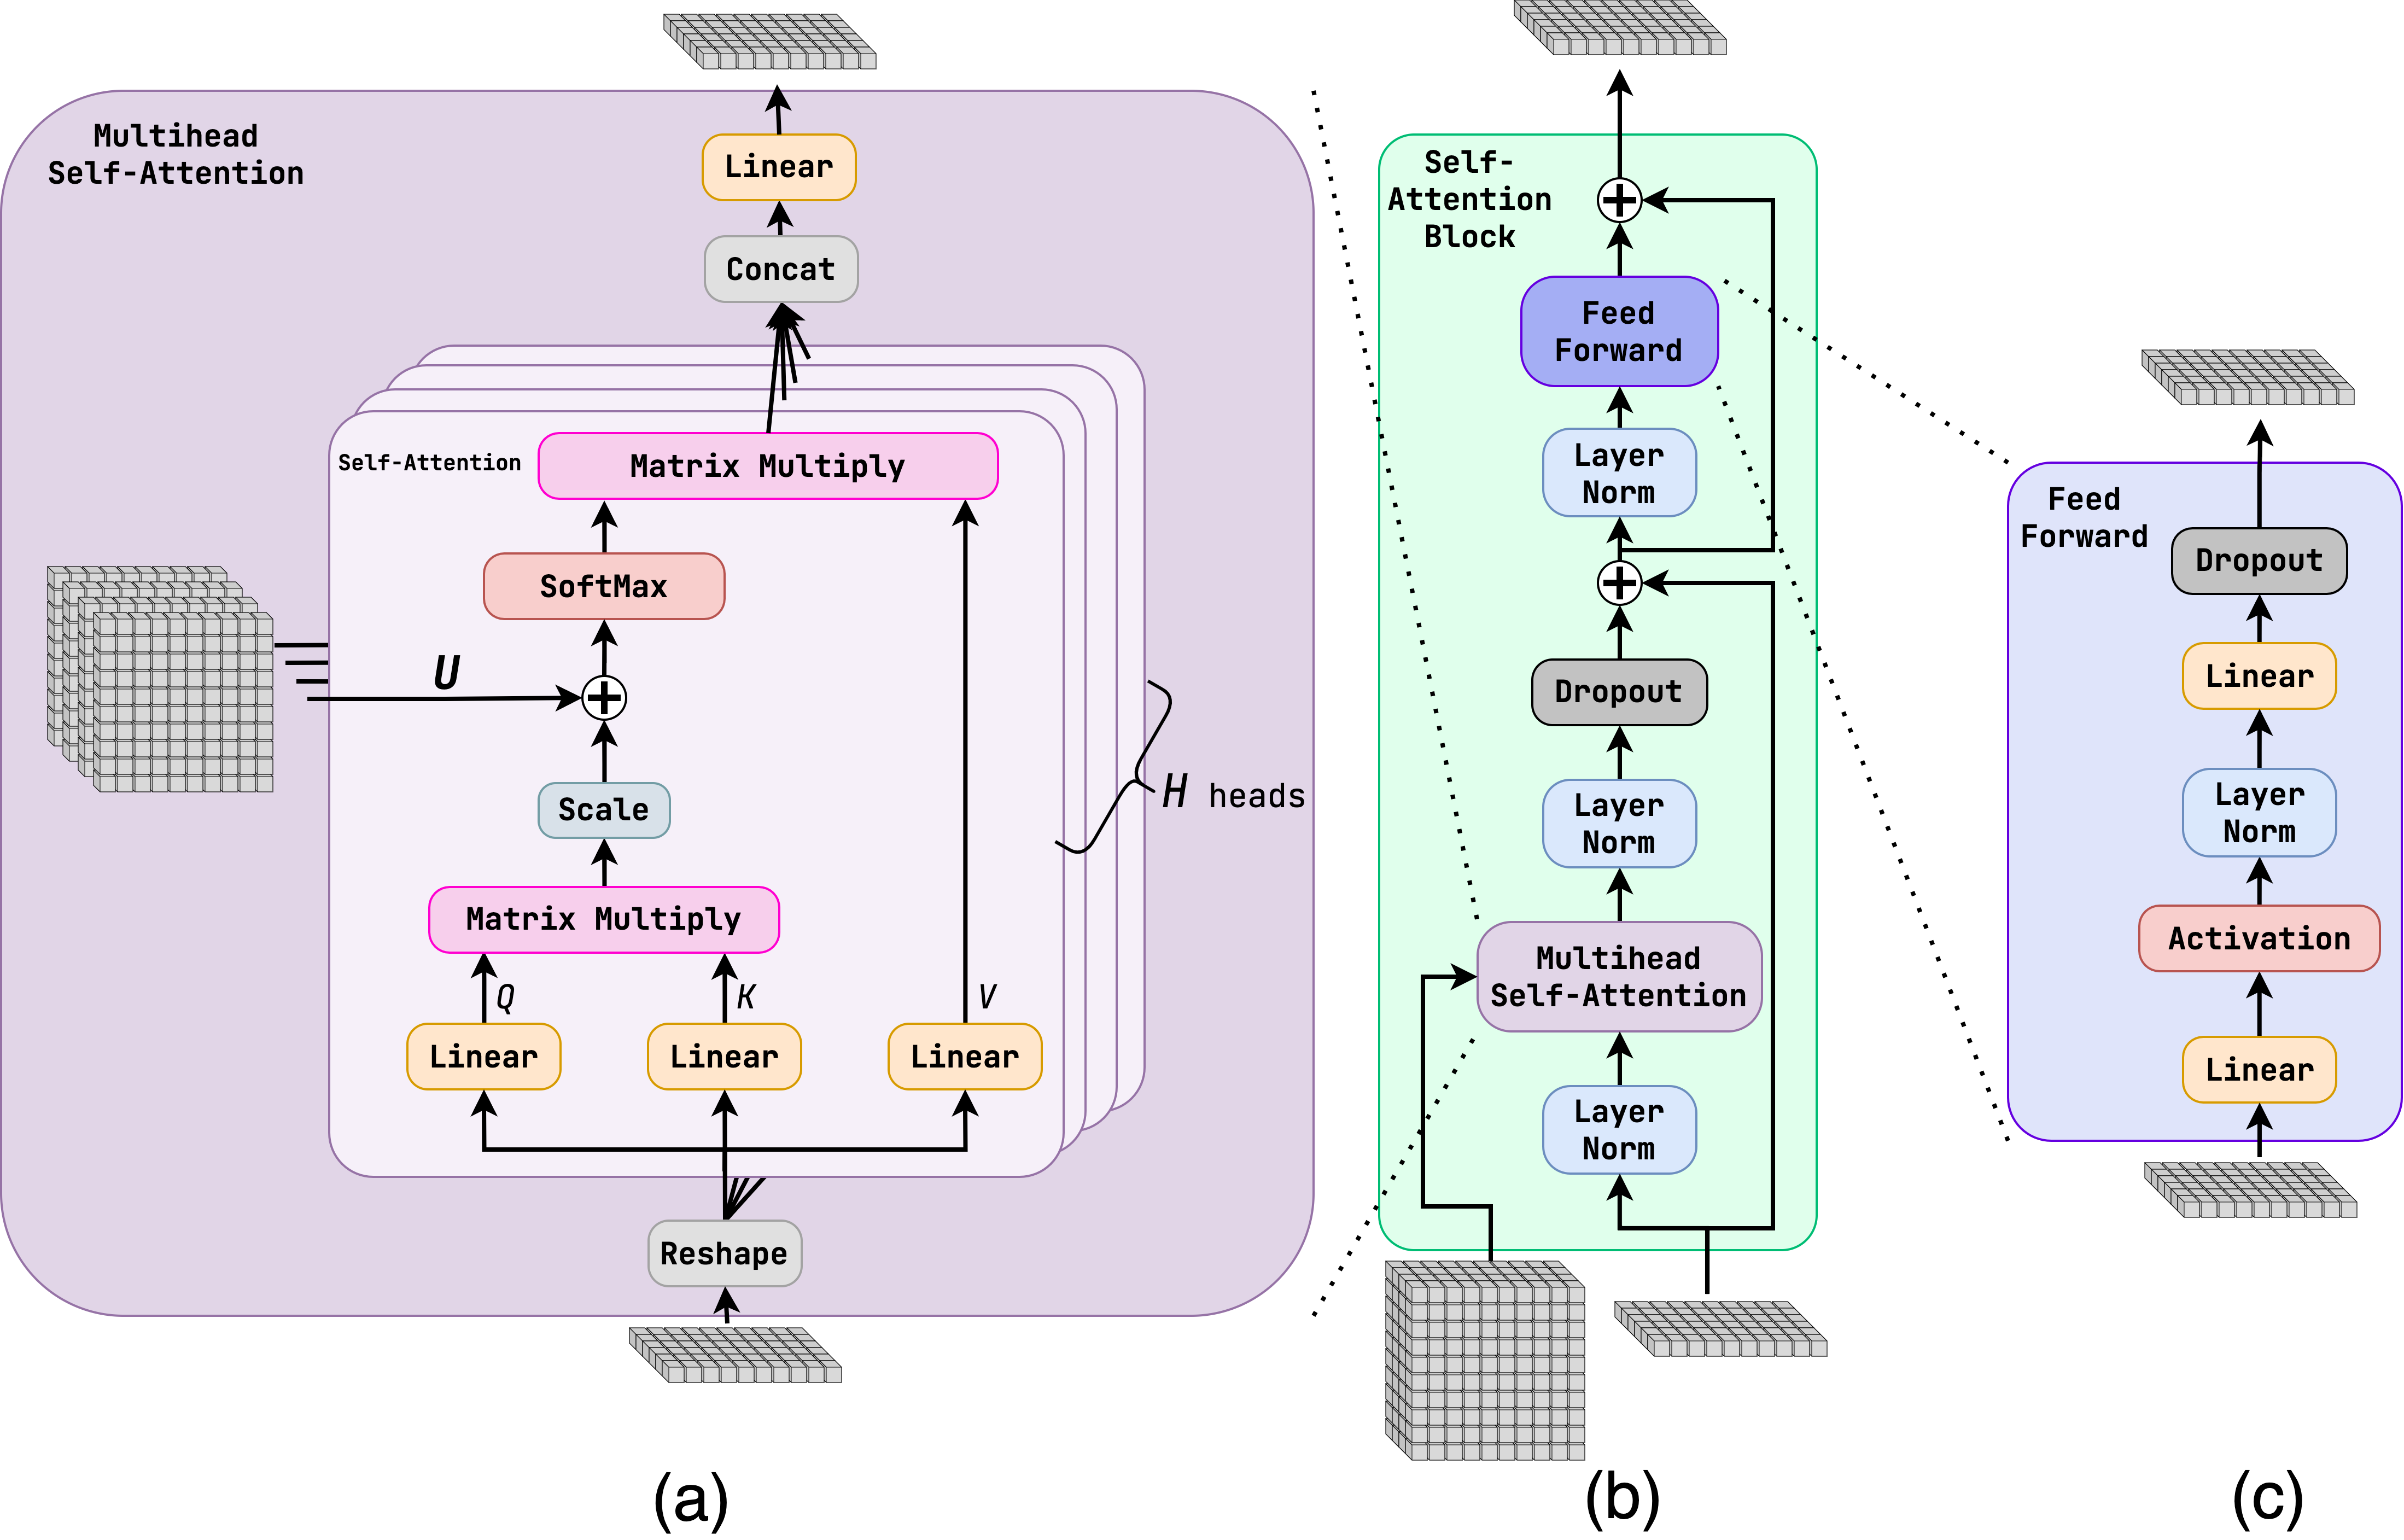
\includegraphics[width=1\linewidth]{src/diagrams/part_layers_1.png}
    \caption{Self-Attention layers of Particle Transformer.}
    \label{fig:part_SA}
\end{figure}

\begin{figure}[htb]
    \centering
    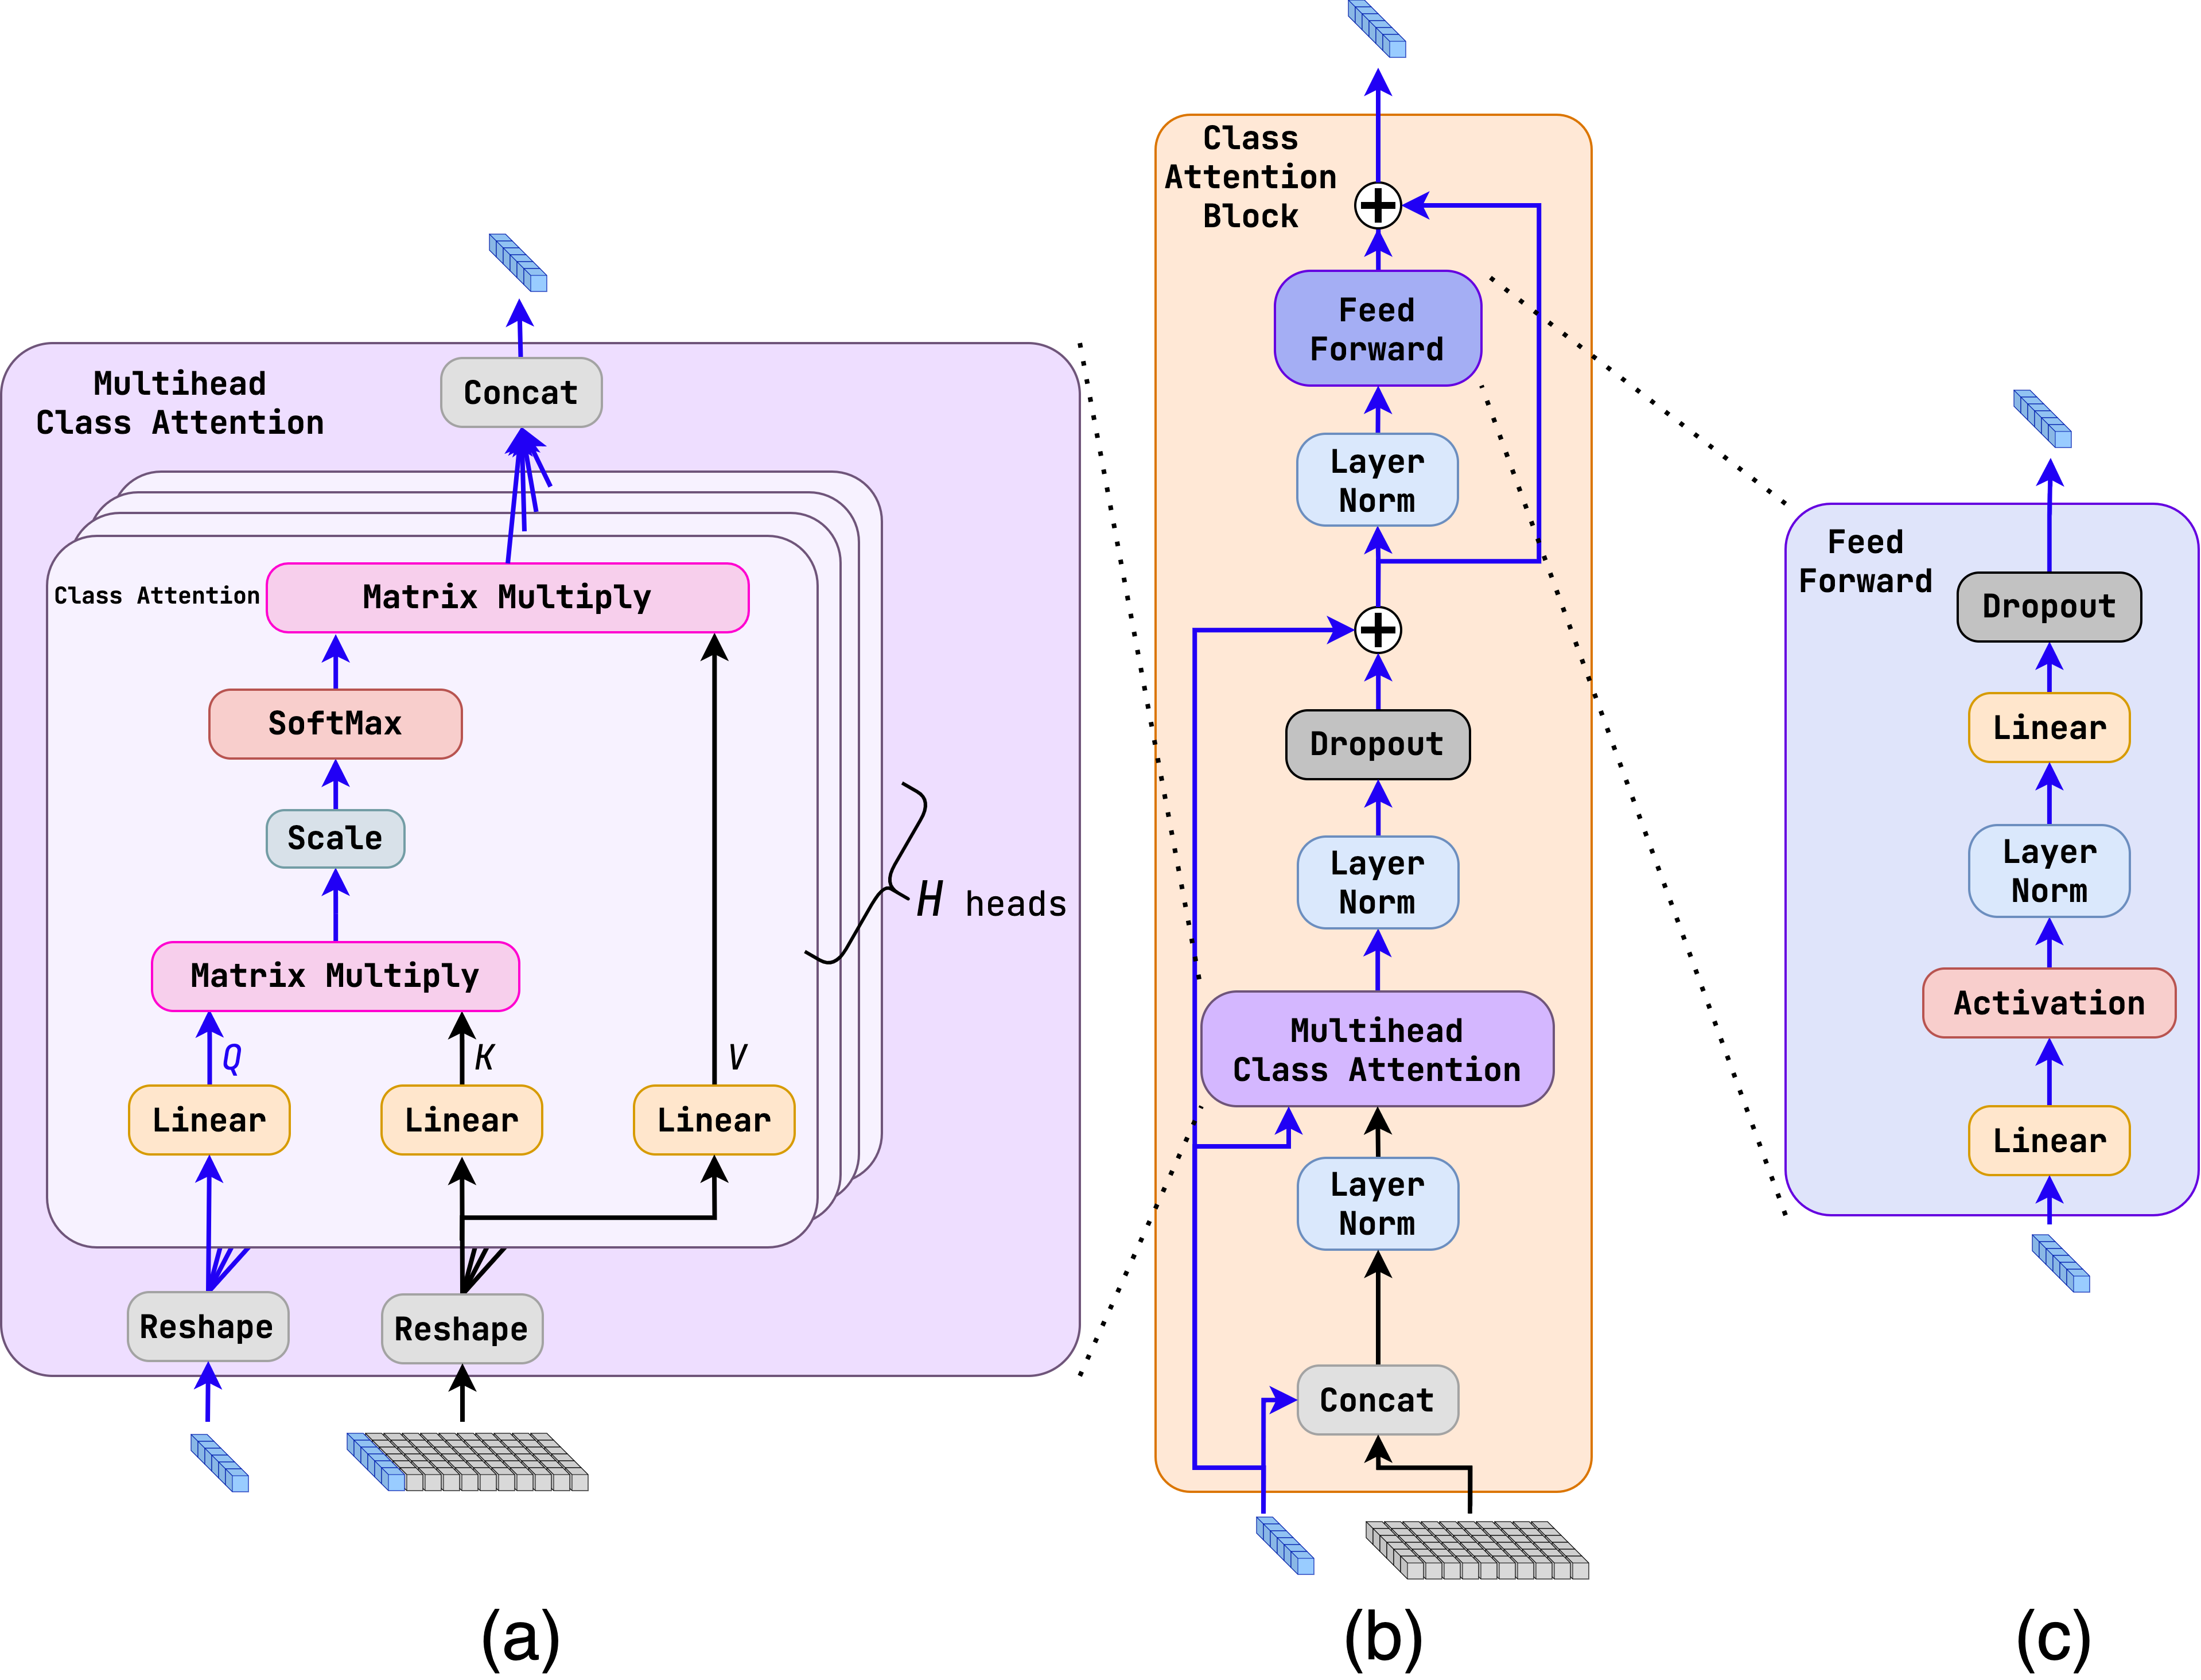
\includegraphics[width=1\linewidth]{src/diagrams/part_layers_2.png}
    \caption{Class Attention layers of Particle Transformer.}
    \label{fig:part_CA}
\end{figure}

\emph{Particle Transformer} \cite{part} is a \trans variant with particle physics in mind.
It is based on the CaiT \cite{cait} architecture (see \cref{fig:part}) with one crucial extension: \emph{the interaction variables}.
Interaction variables are given for each pair of input vectors, producing an overall second input of shape $B \times N \times N \times C_{int}$, where $C_{int}$ is the number of interaction variables.
These variables are manually engineered\footnote{The explicit form depends on the input type. In the case of PFOs, the variables are shown in \red{[????]}} and embedded using the \emph{CNN embedding}, consisting of multiple blocks of \pointCNN, batch normalization and Activation, as shown in \cref{fig:embed} (b).
Since the variables are symmetric, we only need to embed the upper triangle of the matrix, and the lower triangle is filled with the transposed upper triangle.
The diagonal is filled with zeros.

Afterward, they are used as the second input \emph{to every} \SA Block, which is shown in \cref{fig:part,fig:part_SA}, to modify the Attention as
\begin{equation}
    \label{eq:attn_mod}
    \text{\texttt{Attention}} = \text{softmax}\left(\frac{QK^T}{\sqrt{d}} + U\right),
\end{equation}
where $U$ is embedded interaction variables.
The \pointCNN embedding of interaction variables is done into $H$ (number of heads) dimensions, resulting in a matrix of shape $B \times N \times N \times H$ providing each head with its own interaction variables matrix $U$ of shape $B \times N \times N$.

The only difference between \SA Blocks in \trans and \ParT is the addition of two \LN, right after the \MHSA and right before the second \texttt{Linear} layer of the \FFN.
However, \ParT utilizes the \CA layer (\cref{sec:CA}) for feature extraction, which is shown in \cref{fig:part} and more detailed in \cref{fig:part_CA}.
It introduces the Class Token later in the architecture, allowing the \MHSA to focus purely on the input data.
The output class is calculated from the Class Token as in \trans.

Utilizing the interaction variables helps the model focus on the input data's essential parts.
Each head of the \MHSA focuses on a different part of the input data.
The improvement of the \ParT with the interaction variables compared to one without them is significant \cite{part} (see \red{[????]}).
On top of that, the \CA blocks allow a more complex representation of \PFOs and the jet information by separating the attention mechanisms.

\subsection{Class Attention Block}
\label{sec:CA}
\emph{Class Attention Block} (CA Block) is a \MHA layer with the \emph{Class Token as the query}.
The input of the \CA Block is a set of vectors of shape $B \times N \times C$ and the Class Token of shape $B \times C$. 
The Class Token is concatenated to this set of vectors, resulting in a tensor of shape $B \times (N+1) \times C$, and used as a query for the \MHA, as seen in \cref{fig:part_CA}.
This allows the model to focus on the class information. 
The Class Token asks for it and stores it.

Carrying out the matrix multiplications of the \MHA yields a tensor of the same shape as the Class Token, i.e., a vector of shape $B \times C$.
This vector is then pushed through the \FFN, outputting a vector of 'attended' Class Token.
The residual connections use only the Class Token.
The traces of the Class Token are displayed as blue arrows in \cref{fig:part_CA}.

Two \CA Blocks are put after the \SA Blocks, both having the same input of the set of vectors, and the output of the first \CA Block is used as the Class Token input for the second \CA Block.
The second \CA Block output is a vector of shape $B \times C$, with the extracted information about the class of the entire input, which is then passed through a \texttt{Linear} layer to get the final output followed by sigmoid or softmax Activation.



\section{Dynamically Enhanced Particle Transformer}
\label{sec:depart}

\begin{figure}[htb]
    \centering
    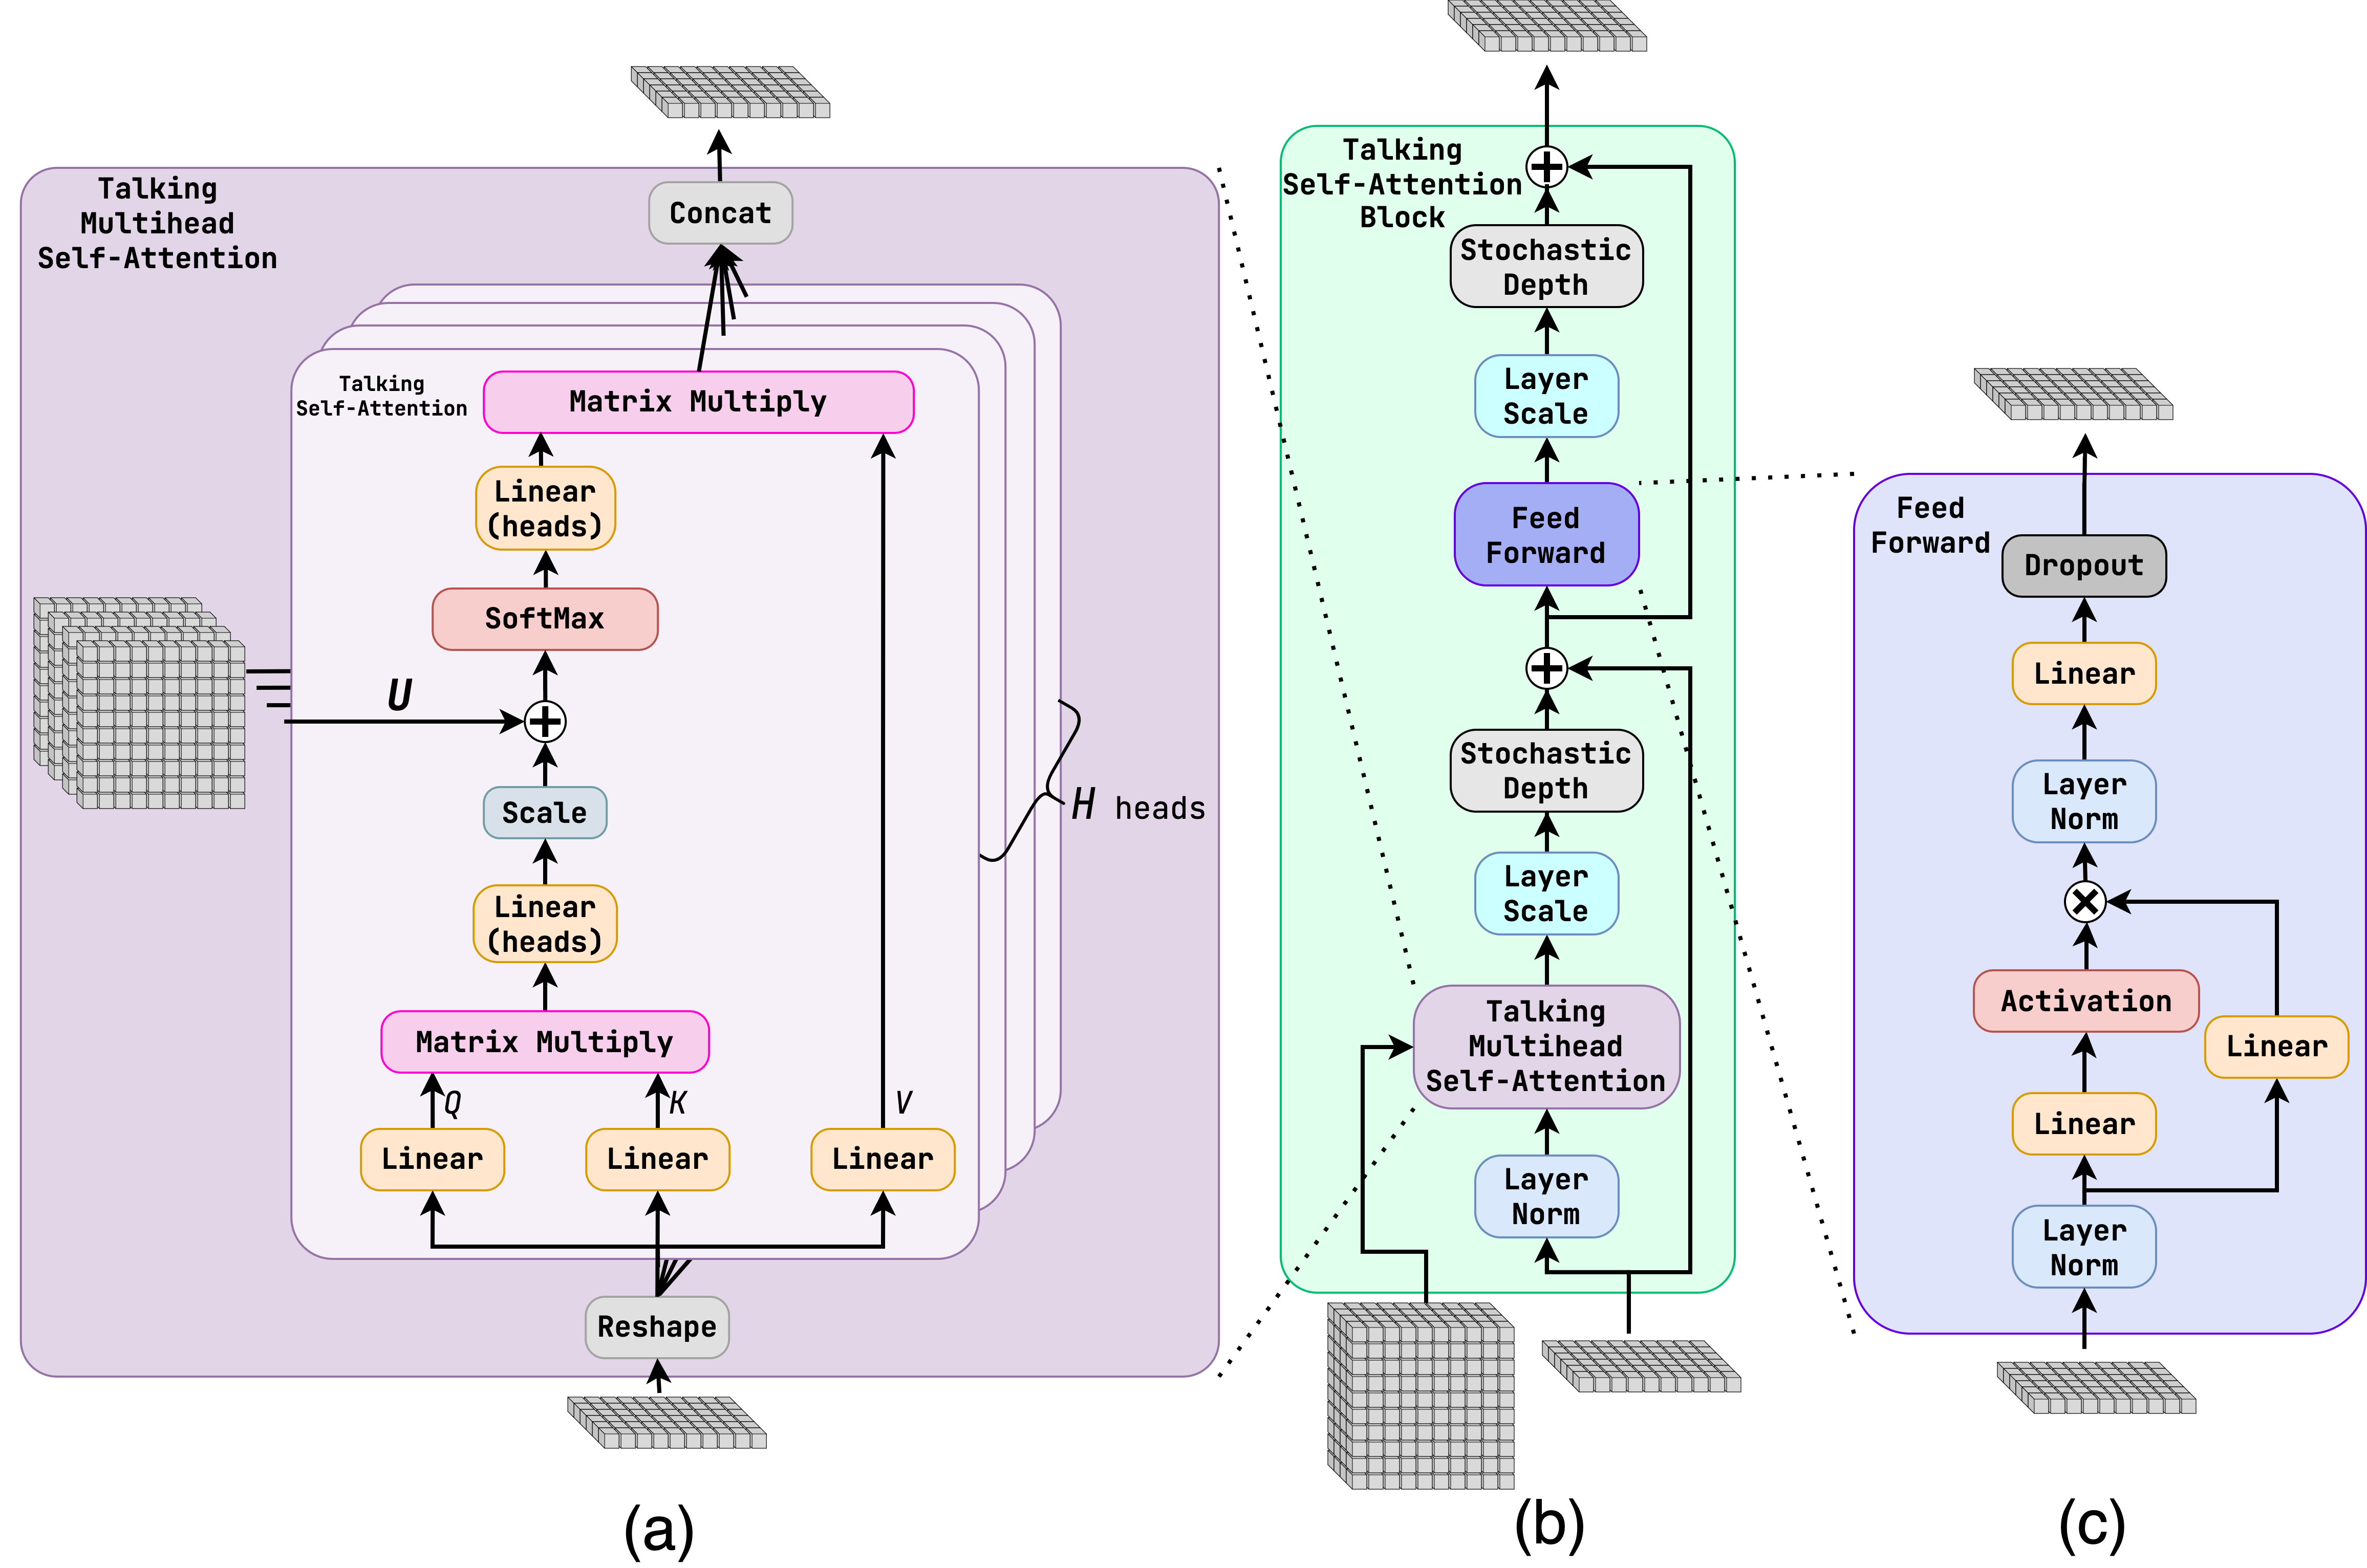
\includegraphics[width=1\linewidth]{src/diagrams/depart_layers.png}
    \caption{Talking Self-Attention layers of Dynamically Enhanced Particle Transformer.}
    \label{fig:depart_SA}
\end{figure}


The \emph{Dynamically Enhanced Particle Transformer} (DeParT) is an enhancement of the \ParT architecture, utilizing the \emph{Talking Multi-Head Attention} \cite{deit3} mechanism (\cref{sec:talk_SA}).
Other improvements include the use of \emph{Stochastic Depth} (\cref{sec:stoch_depth}), \emph{Layer Scale} (\cref{sec:layer_scale}), and \emph{gated} \FFN (\cref{sec:gated_ffn}), all visualized together in \cref{fig:depart_SA}.
The overall structure of the model is the same as in \cref{fig:part}, but the \SA Blocks are replaced with \emph{Talking Self-Attention Blocks} (see \cref{sec:talk_SA}).
The only modifications of \CA Blocks are the replacements of classical \FFN with gated \FFN.

The \emph{Talking Multihead Self-Attention} utilizes the \emph{interaction variables} even more by allowing the heads to exchange information about a given feature each head possesses.
On top of that, the \emph{Layer Scale} and \emph{Stochastic Depth} allow us to train bigger models.

\subsection{Talking Self-Attention Block}
\label{sec:talk_SA}
The \emph{Talking Self-Attention Block} \cite{deit3} is an extension of the \MHA, allowing individual heads to \emph{talk} to each other.
This is done by doing a linear projection across the heads, in other words, applying a \texttt{Linear} layer across the heads dimension $H$. 
We do this twice in the \MHA, right after the matrix multiplication of the query and key and right before the matrix multiplication of the value and the attention weights, as shown in \cref{fig:depart_SA}.

\subsection{Stochastic Depth}
\label{sec:stoch_depth}
\emph{Stochastic Depth} \cite{stoch_depth} is a type of dropout, whose \emph{probability is dependent} on the layer number and drops the \emph{entire layer} rather than individual elements of the output.
The deeper the layer, the bigger the probability of dropping it, linearly dependent as
\begin{equation}
    \label{eq:stoch_depth}
    p_l = \frac{p_L}{2} \cdot \left(1 + \frac{l}{L}\right),
\end{equation}
$p_L$ is the probability of dropping the last layer, $L$ is the total number of layers, and $l$ is the current layer number.
The first layer is indexed as $l=0$.

Each Talking Self-Attention Block is the Stochastic Depth applied twice, after the \MHSA and the \FFN.

\subsection{Layer Scale}
\label{sec:layer_scale}
\emph{Layer Scale} \cite{cait} is a type of normalization that helps the convergence of Transformers with many layers. 
Residual connections cause a bottleneck in the flow of gradients.
This can be prevented by scaling the outputs of \SA and \FFN by an diagonal matrix $\operatorname{diag}\left(\lambda_{l, 1}, \ldots, \lambda_{l, d}\right)$
\begin{equation}
\begin{aligned}
    x_l^{\prime} & =x_l+\operatorname{diag}\left(\lambda_{l, 1}, \ldots, \lambda_{l, d}\right) \times \operatorname{SA}\left(\operatorname{LN}\left(x_l\right)\right), \\
    x_{l+1} & =x_l^{\prime}+\operatorname{diag}\left(\lambda_{l, 1}^{\prime}, \ldots, \lambda_{l, d}^{\prime}\right) \times \operatorname{FFN}\left(\operatorname{LN}\left(x_l^{\prime}\right)\right),
\end{aligned}
\end{equation}
where $x_l$ is the input of the layer, $x_l^{\prime}$ is the output of the \SA layer, and $x_{l+1}$ is the output of the \FFN layer.
The parameters $\lambda_{l, i}$ and $\lambda_{l, i}^{\prime}$ are learned during the training, but at the beginning, are initialized with small values (e.g., $10^{-5}$).

Layer Scale is applied after the \SA and \FFN layers in every \SA Block.

\subsection{Gated Feed-Forward Network}
\label{sec:gated_ffn}
\emph{Gated Feed-Forward Network} is a type of \FFN, which uses a \GLU \cite{GLU}.
Rather than being an improvement of the \FFN, it is an improvement of the Activation after a linear layer.
We can express the \GLU in the form
\begin{equation}
    \pmb{o} = f(\pmb{W} \pmb{x}) \cdot \pmb{W}_{\text{g}} \pmb{x},
\end{equation}
where $\pmb{o}$ is the output, $\pmb{x}$ is the input, $\pmb{W}$ are the weights of the linear layer, $\pmb{W}_g$ are the \emph{weights of the gate} of the same shape as $\pmb{W}$, and $f$ is the activation function.
We apply the ReLU activation in all gated \FFN since it is the best performing \cite{GLU}.
There is also no bias in the \GLU, which makes the model perform better.

By introducing the second weight matrix $\pmb{W}_g$, the overall size of the \FFN would be bigger.
To have the same size as the classical \FFN, the layer expansion is multiplied by the factor of $2/3$.


